% ============================================================
% MPhil thesis, Robotics and Autonomous Systems Thrust, HKUST(GZ)
% Template: github.com/crimson-and-clover/hkustgz-thesis-template (MIT), adjusted to the
% FYTGS(GZ) Guidelines on Thesis Preparation (22 Jan 2024) and the MPhil sample pages (Mar 2024):
% page order, 12 pt, one-and-a-half spacing, 25 mm margins, centred page numbers, abstract <= 300 words.
% Build:  bash sync_from_paper.sh && tectonic -X compile main.tex
% ============================================================
\documentclass[a4paper]{template/hkustgz-thesis}
\usepackage{xspace}
\usepackage{enumitem}
\newcommand{\ours}{S2M\xspace}
\newcommand{\checkme}[1]{\textcolor{red}{#1}}  % fields the author must confirm before submission
\newcommand{\nEBThree}{55.0}
\newcommand{\nEBThreeLo}{49.3}
\newcommand{\nEBThreeHi}{60.7}
\newcommand{\nEBThreeBase}{66.7}
\newcommand{\nEBThreeCommon}{65.0}
\newcommand{\nEBThreeComplex}{65.0}
\newcommand{\nEBThreeVisual}{53.3}
\newcommand{\nEBThreeLong}{25.0}
\newcommand{\nEBThreeAWQ}{48.0}
\newcommand{\nEBThreeAWQLo}{42.3}
\newcommand{\nEBThreeAWQHi}{53.7}
\newcommand{\nEBThreeAWQBase}{65.0}
\newcommand{\nEBThreeAWQCommon}{65.0}
\newcommand{\nEBThreeAWQComplex}{60.0}
\newcommand{\nEBThreeAWQVisual}{38.3}
\newcommand{\nEBThreeAWQLong}{11.7}
\newcommand{\nSThree}{79.2}
\newcommand{\nSThreeLo}{74.7}
\newcommand{\nSThreeHi}{83.6}
\newcommand{\nSThreeBase}{87.8}
\newcommand{\nSThreeCommon}{83.9}
\newcommand{\nSThreeComplex}{85.0}
\newcommand{\nSThreeVisual}{59.4}
\newcommand{\nSThreeLong}{80.0}
\newcommand{\nRGBThree}{76.5}
\newcommand{\nRGBThreeLo}{71.8}
\newcommand{\nRGBThreeHi}{81.0}
\newcommand{\nRGBThreeBase}{85.0}
\newcommand{\nRGBThreeCommon}{80.8}
\newcommand{\nRGBThreeComplex}{85.8}
\newcommand{\nRGBThreeVisual}{52.5}
\newcommand{\nRGBThreeLong}{78.3}
\newcommand{\nEBTwo}{20.3}
\newcommand{\nEBTwoLo}{16.0}
\newcommand{\nEBTwoHi}{25.0}
\newcommand{\nEBTwoBase}{21.7}
\newcommand{\nEBTwoCommon}{21.7}
\newcommand{\nEBTwoComplex}{28.3}
\newcommand{\nEBTwoVisual}{20.0}
\newcommand{\nEBTwoLong}{10.0}
\newcommand{\nEBTwoAWQ}{6.3}
\newcommand{\nEBTwoAWQLo}{3.7}
\newcommand{\nEBTwoAWQHi}{9.3}
\newcommand{\nEBTwoAWQBase}{6.7}
\newcommand{\nEBTwoAWQCommon}{6.7}
\newcommand{\nEBTwoAWQComplex}{6.7}
\newcommand{\nEBTwoAWQVisual}{8.3}
\newcommand{\nEBTwoAWQLong}{3.3}
\newcommand{\nEBTwoAWQraw}{5.7}
\newcommand{\nEBTwoAWQrawLo}{3.3}
\newcommand{\nEBTwoAWQrawHi}{8.3}
\newcommand{\nEBTwoAWQrawBase}{8.3}
\newcommand{\nEBTwoAWQrawCommon}{6.7}
\newcommand{\nEBTwoAWQrawComplex}{6.7}
\newcommand{\nEBTwoAWQrawVisual}{6.7}
\newcommand{\nEBTwoAWQrawLong}{0.0}
\newcommand{\nSTwo}{70.0}
\newcommand{\nSTwoLo}{64.7}
\newcommand{\nSTwoHi}{75.0}
\newcommand{\nSTwoBase}{78.3}
\newcommand{\nSTwoCommon}{71.7}
\newcommand{\nSTwoComplex}{71.7}
\newcommand{\nSTwoVisual}{53.3}
\newcommand{\nSTwoLong}{75.0}
\newcommand{\nOracle}{91.3}
\newcommand{\nOracleLo}{88.0}
\newcommand{\nOracleHi}{94.3}
\newcommand{\nOracleBase}{93.3}
\newcommand{\nOracleCommon}{93.3}
\newcommand{\nOracleComplex}{93.3}
\newcommand{\nOracleVisual}{93.3}
\newcommand{\nOracleLong}{83.3}
\newcommand{\nModThree}{65.0}
\newcommand{\nModThreeLo}{59.7}
\newcommand{\nModThreeHi}{70.3}
\newcommand{\nModThreeBase}{73.3}
\newcommand{\nModThreeCommon}{63.3}
\newcommand{\nModThreeComplex}{63.3}
\newcommand{\nModThreeVisual}{51.7}
\newcommand{\nModThreeLong}{73.3}
\newcommand{\nGainThree}{24.2}
\newcommand{\nGainThreeLo}{17.6}
\newcommand{\nGainThreeHi}{30.7}
\newcommand{\nGainThreeAbs}{24.2}
\newcommand{\nGainThreeP}{{<}10^{-5}}
\newcommand{\nGainThreeBase}{+21.1}
\newcommand{\nGainThreeCommon}{+18.9}
\newcommand{\nGainThreeComplex}{+20.0}
\newcommand{\nGainThreeVisual}{+6.1}
\newcommand{\nGainThreeLong}{+55.0}
\newcommand{\nGainTwo}{49.7}
\newcommand{\nGainTwoLo}{43.0}
\newcommand{\nGainTwoHi}{56.3}
\newcommand{\nGainTwoAbs}{49.7}
\newcommand{\nGainTwoP}{{<}10^{-5}}
\newcommand{\nGainTwoBase}{+56.7}
\newcommand{\nGainTwoCommon}{+50.0}
\newcommand{\nGainTwoComplex}{+43.3}
\newcommand{\nGainTwoVisual}{+33.3}
\newcommand{\nGainTwoLong}{+65.0}
\newcommand{\nGainRGB}{21.5}
\newcommand{\nGainRGBLo}{14.7}
\newcommand{\nGainRGBHi}{28.2}
\newcommand{\nGainRGBAbs}{21.5}
\newcommand{\nGainRGBP}{{<}10^{-5}}
\newcommand{\nGainRGBBase}{+18.3}
\newcommand{\nGainRGBCommon}{+15.8}
\newcommand{\nGainRGBComplex}{+20.8}
\newcommand{\nGainRGBVisual}{-0.8}
\newcommand{\nGainRGBLong}{+53.3}
\newcommand{\nGainThreeAWQ}{31.2}
\newcommand{\nGainThreeAWQLo}{24.8}
\newcommand{\nGainThreeAWQHi}{37.4}
\newcommand{\nGainThreeAWQAbs}{31.2}
\newcommand{\nGainThreeAWQP}{{<}10^{-5}}
\newcommand{\nGainThreeAWQBase}{+22.8}
\newcommand{\nGainThreeAWQCommon}{+18.9}
\newcommand{\nGainThreeAWQComplex}{+25.0}
\newcommand{\nGainThreeAWQVisual}{+21.1}
\newcommand{\nGainThreeAWQLong}{+68.3}
\newcommand{\nGainTwoAWQ}{63.7}
\newcommand{\nGainTwoAWQLo}{58.0}
\newcommand{\nGainTwoAWQHi}{69.3}
\newcommand{\nGainTwoAWQAbs}{63.7}
\newcommand{\nGainTwoAWQP}{{<}10^{-5}}
\newcommand{\nGainTwoAWQBase}{+71.7}
\newcommand{\nGainTwoAWQCommon}{+65.0}
\newcommand{\nGainTwoAWQComplex}{+65.0}
\newcommand{\nGainTwoAWQVisual}{+45.0}
\newcommand{\nGainTwoAWQLong}{+71.7}
\newcommand{\nQuantThree}{7.0}
\newcommand{\nQuantThreeLo}{0.7}
\newcommand{\nQuantThreeHi}{13.3}
\newcommand{\nQuantThreeAbs}{7.0}
\newcommand{\nQuantThreeP}{{=}0.04}
\newcommand{\nQuantThreeBase}{+1.7}
\newcommand{\nQuantThreeCommon}{+0.0}
\newcommand{\nQuantThreeComplex}{+5.0}
\newcommand{\nQuantThreeVisual}{+15.0}
\newcommand{\nQuantThreeLong}{+13.3}
\newcommand{\nQuantTwo}{14.0}
\newcommand{\nQuantTwoLo}{8.7}
\newcommand{\nQuantTwoHi}{19.3}
\newcommand{\nQuantTwoAbs}{14.0}
\newcommand{\nQuantTwoP}{{<}10^{-5}}
\newcommand{\nQuantTwoBase}{+15.0}
\newcommand{\nQuantTwoCommon}{+15.0}
\newcommand{\nQuantTwoComplex}{+21.7}
\newcommand{\nQuantTwoVisual}{+11.7}
\newcommand{\nQuantTwoLong}{+6.7}
\newcommand{\nGapRGB}{-2.7}
\newcommand{\nGapRGBLo}{-7.2}
\newcommand{\nGapRGBHi}{1.7}
\newcommand{\nGapRGBAbs}{2.7}
\newcommand{\nGapRGBP}{{=}0.24}
\newcommand{\nGapRGBBase}{-2.8}
\newcommand{\nGapRGBCommon}{-3.1}
\newcommand{\nGapRGBComplex}{+0.8}
\newcommand{\nGapRGBVisual}{-6.9}
\newcommand{\nGapRGBLong}{-1.7}
\newcommand{\nGapOracle}{12.1}
\newcommand{\nGapOracleLo}{7.7}
\newcommand{\nGapOracleHi}{16.8}
\newcommand{\nGapOracleAbs}{12.1}
\newcommand{\nGapOracleP}{{<}10^{-5}}
\newcommand{\nGapOracleBase}{+5.6}
\newcommand{\nGapOracleCommon}{+9.4}
\newcommand{\nGapOracleComplex}{+8.3}
\newcommand{\nGapOracleVisual}{+33.9}
\newcommand{\nGapOracleLong}{+3.3}
\newcommand{\nModOverEB}{10.0}
\newcommand{\nModOverEBLo}{2.3}
\newcommand{\nModOverEBHi}{17.7}
\newcommand{\nModOverEBAbs}{10.0}
\newcommand{\nModOverEBP}{{=}0.01}
\newcommand{\nModOverEBBase}{+6.7}
\newcommand{\nModOverEBCommon}{-1.7}
\newcommand{\nModOverEBComplex}{-1.7}
\newcommand{\nModOverEBVisual}{-1.7}
\newcommand{\nModOverEBLong}{+48.3}
\newcommand{\nSOverMod}{14.2}
\newcommand{\nSOverModLo}{9.0}
\newcommand{\nSOverModHi}{19.6}
\newcommand{\nSOverModAbs}{14.2}
\newcommand{\nSOverModP}{{<}10^{-5}}
\newcommand{\nSOverModBase}{+14.4}
\newcommand{\nSOverModCommon}{+20.6}
\newcommand{\nSOverModComplex}{+21.7}
\newcommand{\nSOverModVisual}{+7.8}
\newcommand{\nSOverModLong}{+6.7}
\newcommand{\nMcNThreeWorst}{{=}2.2{\times}10^{-11}}
\newcommand{\nMcNTwoWorst}{{=}2.3{\times}10^{-33}}
\newcommand{\nMcNRGBWorst}{{=}5.2{\times}10^{-9}}
\newcommand{\nDiscTwoWins}{163}
\newcommand{\nDiscTwoLosses}{14}
\newcommand{\nDiscTwoP}{{=}2.3{\times}10^{-33}}
\newcommand{\nDiscThreeWins}{95}
\newcommand{\nDiscThreeLosses}{20}
\newcommand{\nDiscThreeP}{{=}7.1{\times}10^{-13}}
\newcommand{\nDiscGlobalWins}{59}
\newcommand{\nDiscGlobalLosses}{65}
\newcommand{\nDiscGlobalP}{{=}0.65}
\newcommand{\nRGBGlobal}{53.0}
\newcommand{\nGainGlobal}{-2.0}
\newcommand{\nVisDiffLo}{-9.4}
\newcommand{\nVisDiffHi}{+21.7}
\newcommand{\nVisDiffP}{{=}0.49}
\newcommand{\nQuantThreeNamedMax}{+5.0}
\newcommand{\nQuantThreeWins}{58}
\newcommand{\nQuantThreeLosses}{37}
\newcommand{\nQuantTwoWins}{58}
\newcommand{\nQuantTwoLosses}{16}
\newcommand{\nSThreeSD}{0.7}
\newcommand{\nRGBThreeSD}{0.2}
\newcommand{\nSThreeMin}{78.7}
\newcommand{\nSThreeMax}{80.0}
\newcommand{\nScaleDrop}{9.2}
\newcommand{\nScaleDropEB}{34.7}
\newcommand{\nOracleGapLong}{3.3}
\newcommand{\nStepN}{141}
\newcommand{\nStepS}{10.8}
\newcommand{\nStepEB}{12.6}
\newcommand{\nStepRed}{14}
\newcommand{\nStepFewer}{86}
\newcommand{\nStepMore}{29}
\newcommand{\nStepP}{{=}9.8{\times}10^{-8}}
\newcommand{\nTokS}{9.0}
\newcommand{\nTokSc}{383}
\newcommand{\nCallsS}{31.4}
\newcommand{\nTokEB}{27.1}
\newcommand{\nTokEBc}{2.3}
\newcommand{\nCallsEB}{7.8}
\newcommand{\nEBThreeParse}{1 of its 2,342 replies cannot be parsed and is replaced by a random action, as in the benchmark}
\newcommand{\nFailEBThree}{135}
\newcommand{\nNeverEBThree}{12}
\newcommand{\nLostEBThree}{43}
\newcommand{\nNearEBThree}{34}
\newcommand{\nBlockedEBThree}{26}
\newcommand{\nFailSThree}{62.3}
\newcommand{\nNeverSThree}{1.3}
\newcommand{\nLostSThree}{20.7}
\newcommand{\nNearSThree}{9.3}
\newcommand{\nBlockedSThree}{2.7}
\newcommand{\nLostEBTwo}{104}
\newcommand{\nLostSTwo}{48}
\newcommand{\nNeverLongEBThree}{12}
\newcommand{\nRecallOtherLo}{92}
\newcommand{\nRecallOtherHi}{97}
\newcommand{\nRecallVisLo}{65}
\newcommand{\nRecallVisHi}{68}
\newcommand{\nVisFail}{73}
\newcommand{\nVisFailNoCand}{46}
\newcommand{\nVisSRLo}{56.7}
\newcommand{\nVisSRHi}{61.7}
\newcommand{\nProbeThreeBase}{78.7}
\newcommand{\nProbeThreeCommon}{69.3}
\newcommand{\nProbeThreeComplex}{77.3}
\newcommand{\nProbeThreeVisual}{49.3}
\newcommand{\nProbeTwoBase}{40.0}
\newcommand{\nProbeTwoCommon}{33.3}
\newcommand{\nProbeTwoComplex}{37.3}
\newcommand{\nProbeTwoVisual}{18.7}
\newcommand{\nFalseBoxNamedLo}{15}
\newcommand{\nFalseBoxNamedHi}{19}
\newcommand{\nFalseBoxVisual}{41}
\newcommand{\nDetPrec}{77}
\newcommand{\nHoldS}{254}
\newcommand{\nHoldNF}{264}
\newcommand{\nLostNF}{42}
\newcommand{\nNearNF}{20}
\newcommand{\nDRmean}{0.10}
\newcommand{\nDRfinal}{0.15}
\newcommand{\nRangeSensor}{0.97}
\newcommand{\nRangeGlobal}{0.90}
\newcommand{\nRangeFloor}{0.93}
\newcommand{\nShortGlobal}{66}
\newcommand{\nShortFloor}{10.0}
\newcommand{\nProbeViews}{240}
\newcommand{\nBlockGlobal}{42.5}
\newcommand{\nBlockFloor}{9.9}
\newcommand{\nAbsRelGlobal}{0.134}
\newcommand{\nAbsRelFloor}{0.115}
\newcommand{\nShortSensorMax}{0}
\newcommand{\nVisGapShare}{56}
\newcommand{\nCapAWQ}{14.8}
\newcommand{\nIdFirstAWQ}{92.6}
\newcommand{\nIdLaterAWQ}{79.3}
\newcommand{\nCapFP}{3.2}
\newcommand{\nIdFirstFP}{99.6}
\newcommand{\nIdLaterFP}{95.7}
\newcommand{\nRoboN}{1800}
\newcommand{\nRoboSR}{59.6}
\newcommand{\nRoboSRLo}{57.3}
\newcommand{\nRoboSRHi}{61.8}
\newcommand{\nRoboSPL}{35.9}
\newcommand{\nRoboSPLLo}{34.2}
\newcommand{\nRoboSPLHi}{37.6}
\newcommand{\nRoboBest}{88.0}
\newcommand{\nRoboWorst}{25.3}
\newcommand{\nRoboErr}{17}
\newcommand{\nAblFusion}{-8.6}
\newcommand{\nAblFusionAbs}{8.6}
\newcommand{\nAblFusionLo}{-12.7}
\newcommand{\nAblFusionHi}{-4.6}
\newcommand{\nAblFusionP}{{=}3.4{\times}10^{-4}}
\newcommand{\nAblFusionBase}{-9.4}
\newcommand{\nAblFusionCommon}{-8.9}
\newcommand{\nAblFusionComplex}{-6.7}
\newcommand{\nAblFusionVisual}{-16.1}
\newcommand{\nAblFusionLong}{-1.7}
\newcommand{\nAblFusionOtherMin}{-16.1}
\newcommand{\nAblFusionOtherMax}{-6.7}
\newcommand{\nAblScan}{0.1}
\newcommand{\nAblScanAbs}{0.1}
\newcommand{\nAblScanLo}{-4.2}
\newcommand{\nAblScanHi}{4.6}
\newcommand{\nAblScanP}{{=}1.00}
\newcommand{\nAblScanBase}{+7.2}
\newcommand{\nAblScanCommon}{+6.1}
\newcommand{\nAblScanComplex}{+6.7}
\newcommand{\nAblScanVisual}{+13.9}
\newcommand{\nAblScanLong}{-33.3}
\newcommand{\nAblScanOtherMin}{+6.1}
\newcommand{\nAblScanOtherMax}{+13.9}
\newcommand{\nAblExhaust}{-1.6}
\newcommand{\nAblExhaustAbs}{1.6}
\newcommand{\nAblExhaustLo}{-3.6}
\newcommand{\nAblExhaustHi}{0.3}
\newcommand{\nAblExhaustP}{{=}0.61}
\newcommand{\nAblExhaustBase}{-1.1}
\newcommand{\nAblExhaustCommon}{-2.2}
\newcommand{\nAblExhaustComplex}{+0.0}
\newcommand{\nAblExhaustVisual}{-1.1}
\newcommand{\nAblExhaustLong}{-3.3}
\newcommand{\nAblExhaustOtherMin}{-2.2}
\newcommand{\nAblExhaustOtherMax}{+0.0}
\newcommand{\nAblZoom}{-4.6}
\newcommand{\nAblZoomAbs}{4.6}
\newcommand{\nAblZoomLo}{-7.9}
\newcommand{\nAblZoomHi}{-1.3}
\newcommand{\nAblZoomP}{{=}0.04}
\newcommand{\nAblZoomBase}{-6.1}
\newcommand{\nAblZoomCommon}{-5.6}
\newcommand{\nAblZoomComplex}{-5.0}
\newcommand{\nAblZoomVisual}{-1.1}
\newcommand{\nAblZoomLong}{-5.0}
\newcommand{\nAblZoomOtherMin}{-6.1}
\newcommand{\nAblZoomOtherMax}{-1.1}
\newcommand{\nAblOdom}{0.1}
\newcommand{\nAblOdomAbs}{0.1}
\newcommand{\nAblOdomLo}{-3.6}
\newcommand{\nAblOdomHi}{3.8}
\newcommand{\nAblOdomP}{{=}1.00}
\newcommand{\nAblOdomBase}{+3.9}
\newcommand{\nAblOdomCommon}{-2.2}
\newcommand{\nAblOdomComplex}{+5.0}
\newcommand{\nAblOdomVisual}{-9.4}
\newcommand{\nAblOdomLong}{+3.3}
\newcommand{\nAblOdomOtherMin}{-9.4}
\newcommand{\nAblOdomOtherMax}{+5.0}
\newcommand{\nAblRgbglobal}{-26.2}
\newcommand{\nAblRgbglobalAbs}{26.2}
\newcommand{\nAblRgbglobalLo}{-32.3}
\newcommand{\nAblRgbglobalHi}{-19.8}
\newcommand{\nAblRgbglobalP}{{<}10^{-5}}
\newcommand{\nAblRgbglobalBase}{-31.1}
\newcommand{\nAblRgbglobalCommon}{-25.6}
\newcommand{\nAblRgbglobalComplex}{-25.0}
\newcommand{\nAblRgbglobalVisual}{-22.8}
\newcommand{\nAblRgbglobalLong}{-26.7}
\newcommand{\nAblRgbglobalOtherMin}{-31.1}
\newcommand{\nAblRgbglobalOtherMax}{-22.8}
\newcommand{\nAblRgbfloor}{-2.7}
\newcommand{\nAblRgbfloorAbs}{2.7}
\newcommand{\nAblRgbfloorLo}{-7.2}
\newcommand{\nAblRgbfloorHi}{1.7}
\newcommand{\nAblRgbfloorP}{{=}0.73}
\newcommand{\nAblRgbfloorBase}{-2.8}
\newcommand{\nAblRgbfloorCommon}{-3.1}
\newcommand{\nAblRgbfloorComplex}{+0.8}
\newcommand{\nAblRgbfloorVisual}{-6.9}
\newcommand{\nAblRgbfloorLong}{-1.7}
\newcommand{\nAblRgbfloorOtherMin}{-6.9}
\newcommand{\nAblRgbfloorOtherMax}{+0.8}
\newcommand{\nScanLongFull}{21}
\newcommand{\nScanLongAbl}{1}
\newcommand{\nScanLongP}{{=}1.1{\times}10^{-5}}
\newcommand{\nBudEBTen}{16.0}
\newcommand{\nBudEBFifteen}{44.7}
\newcommand{\nBudSTen}{30.9}
\newcommand{\nBudSFifteen}{71.8}
\newcommand{\nBudRGBTen}{22.5}
\newcommand{\nBudRGBFifteen}{62.8}
\newcommand{\nBudOracleTen}{40.0}
\newcommand{\nBudOracleFifteen}{87.0}

\newcommand{\tTimeStepS}{0.83}
\newcommand{\tTimeEpS}{11.4}
\newcommand{\tStepsMeanS}{13.7}
\newcommand{\tTraceSteps}{14}
\newcommand{\tTraceTarget}{AlarmClock}
\newcommand{\tTraceFinalW}{7.66}
\newcommand{\tExcerptRejected}{14}
\newcommand{\tExcerptSteps}{20}
\newcommand{\tExcerptSeen}{never}
\newcommand{\tExcerptSSteps}{11}
\newcommand{\tExcerptSOk}{succeeds}
\newcommand{\tLostSVisual}{15.2}
\newcommand{\tLostSAll}{28.5}

\newcommand{\tRStop}{1362}
\newcommand{\tRStopOk}{1072}
\newcommand{\tRStopPrec}{78.7}
\newcommand{\tRWrong}{290}
\newcommand{\tRWrongNear}{45}
\newcommand{\tRWrongDist}{3.6}
\newcommand{\tRLimit}{421}
\newcommand{\tRStepsSucc}{50}
\newcommand{\tRCallsEp}{572}
\newcommand{\tRLimitAppr}{307}
\newcommand{\tRLimitRej}{386}
\newcommand{\tRLimitExpl}{65}
\newcommand{\tRTimeStep}{0.60}


\title{Ask Small VLMs Only What They Can See: A Semantic-to-Metric Agent for Embodied Navigation}
\author{WAN Yifeng}
\degree[\MPhilabbr]{\MPhil}
\department{Robotics and Autonomous Systems Thrust}
\subject{Robotics and Autonomous Systems}
\advisor{Prof. HUANG Qiang}
\depthead{\checkme{Prof. [Head of Thrust]}}{Robotics and Autonomous Systems Thrust}
\titlepagedate{\checkme{[Month Year]}}
\authdate{\checkme{[DD Month YYYY]}}

\addbibresource{references.bib}
\addbibresource{references_thesis.bib}

\begin{document}

% ---- preliminary pages, numbered in lowercase Roman (i is not shown on the title page) ----
\maketitle
\setcounter{page}{2}  % the title page is page i (not shown); the authorization page is ii
\makeauthorization
\makesignature

\begin{acknowledgments}
I am deeply grateful to my supervisor, Prof. HUANG Qiang, for his guidance, encouragement, and patience throughout
my MPhil study. His advice shaped both the questions this thesis asks and the way it answers them. I also thank the
members of my Program Planning cum Thesis Supervision Committee for their time and their comments on this work.

Declaration of assistance: an AI assistant (Claude, Anthropic) was used extensively under my direction to write
and run the experiment code, analyse the results, prepare the figures, and draft and edit the text of this
thesis. The research direction, the choice of benchmarks and robot platform, and the decisions on what to report
are mine. All reported numbers are computed by scripts from the saved experiment records. No other person
provided assistance beyond the supervision acknowledged above.

I thank my colleagues and friends for many discussions, and my family for their constant support.

\end{acknowledgments}

\clearpage
\addcontentsline{toc}{chapter}{Table of Contents}
\tableofcontents
\clearpage
\addcontentsline{toc}{chapter}{List of Figures}
\listoffigures
\clearpage
\addcontentsline{toc}{chapter}{List of Tables}
\listoftables

\begin{abstract}
Robots that follow natural-language instructions need vision-language models (VLMs) small enough to run on board,
yet multimodal language-model agents navigate well only with frontier-scale models. These agents give one model
every role: it reads the image and its own history, keeps track of the room, and writes the plan.

A controlled diagnosis on the EB-Navigation benchmark shows that small VLMs fail because of this role, not
because of perception. Prompted as the benchmark's agent, Qwen3-VL-4B solves \nEBThree\% of the test episodes, whereas a
geometric planner given the target position solves \nOracle\% of the same episodes, and the model boxes a visible
target in \nProbeThreeCommon--\nProbeThreeBase\% of single views. What fails is keeping spatial state in generated
text.

The thesis therefore proposes the Semantic-to-Metric (\ours) agent, which uses the VLM as a sensor rather than a
planner. \ours asks the model only what the current image can answer, whether the target is
visible and where, and keeps all state in metric form. A hypothesis memory lifts each answer with depth and pose,
accumulates evidence across distinct viewpoints, and withdraws it when a hypothesis should be visible but is not
detected; a search policy and an occupancy-map planner compute every move.

Without training and with the model at 4-bit on one 8\,GB GPU, \ours succeeds in \nSThree\% of the EB-Navigation
test episodes, \nGainThree{} percentage points more than the benchmark's agent and \nSOverMod{} more than a generic
modular agent with the same model. From RGB alone, with a per-frame ground-plane scale for monocular depth, it
reaches \nRGBThree\%, above both fine-tuned 4B agents and seven of ten training-free agents built on larger models.
With Qwen2.5-VL-3B, success rises from \nEBTwo\% to \nSTwo\%, and on RoboTHOR object navigation \ours reaches
\nRoboSR\%.

\end{abstract}

% ---- thesis body, numbered in Arabic from the first page of Chapter 1 ----
\mainmatter

\chapter{Introduction}
\label{chap:intro}

\section{Background}
\label{sec:intro-background}
A household robot that is asked to ``find something to heat my lunch'' must solve two problems at once. It must
ground an open-ended instruction in what its camera sees, deciding that a microwave or a toaster satisfies the
request, and it must move through a room it does not know until it reaches that object. The two problems have
historically been studied by different communities with different tools.

Classical mobile robotics solves the second problem well. Occupancy grids~\cite{elfes1989occupancy} turn range
measurements into a probabilistic map of free and occupied space, frontier exploration~\cite{yamauchi1997frontier}
drives the robot toward the boundary between known and unknown space, and graph search such as A*~\cite{hart1968astar}
computes collision-free paths on the map. These components are interpretable, need no training data, and are
reliable enough to be the default in deployed robots~\cite{thrun2005probabilistic}. They know where the robot can
go, but not where a ``kettle'' or ``something to sit on'' is.

The first problem, grounding language in perception, was for a long time restricted to fixed object categories.
Vision-language models (VLMs) trained on web-scale image-text pairs changed this: contrastive models and
open-vocabulary detectors recognize objects named in free text~\cite{radford2021clip,minderer2022owlvit,liu2024groundingdino},
and generative VLMs answer questions about images and localize objects described in words~\cite{bai2025qwen25vl,bai2025qwen3vl}.

Multimodal large language models (MLLMs) have since been used as complete embodied agents. EmbodiedBench evaluates
such agents on standard tasks through a common action interface~\cite{yang2025embodiedbench}. In its navigation
benchmark, EB-Navigation, the agent receives an instruction and a first-person camera image and must come within
1\,m of the described object within 20 steps. The benchmark's own agent gives the model every role. At each step
the model reads the current image and the text history of its previous actions, describes what it sees, reasons
about where the target is, and writes a plan of the next actions.

\section{Motivation}
\label{sec:intro-motivation}
The success of this design tracks model size. GPT-4o succeeds in 57.7\% of the EB-Navigation episodes and
InternVL3-78B in 53.7\%, while models of 7--8B reach 20.3--29.3\% overall and 0--5\% on the Long-horizon subset, in
which the target starts behind the agent~\cite{yang2025embodiedbench}. A tenfold larger model of the same family adds
\nScaleQwen--\nScaleIntern{} percentage points.

The gap matters because a robot has good reasons to use a small local model. A model that runs on the robot's own
computer or on a consumer GPU works without a network connection, answers with a predictable latency, keeps camera
images of a private home on the device, and costs nothing per query. The models that fit these constraints today
have a few billion parameters and are quantized to 4 or 8 bits~\cite{lin2024awq}. A robot that must rely on such a
model cannot adopt the agent designs that work with frontier models, because those designs fail with small models.

The question this thesis pursues is whether the failure is a property of small models or a property of how they are
used. If small models fail because they cannot see well enough, the only remedies are larger models or task-specific
training. If they fail because the agent asks them to do something other than seeing, a different agent may make
them work as they are.

\section{Problem statement}
\label{sec:intro-problem}
Existing remedies keep the model in charge of the plan. Training-free agents surround it with memory, reflection,
skill libraries, scene graphs, or tools~\cite{lee2026emho,ma2026brainmem,zhou2026enabling,huang2025esca,ju2026embodiskill},
but the model still reads that context and writes the plan, and the reported gains rely on models of 8B parameters up
to frontier scale. Fine-tuned agents adapt a 4B model to the task~\cite{xie2026sva,jang2026musix} with training data
and compute, and remain below 60\% on EB-Navigation. Modular object-navigation systems keep a metric map and a
planner~\cite{gadre2022cows,yokoyama2023vlfm,yin2024online}, but they rely on dedicated detectors for fixed
categories, often together with a large language model that decides where to explore.

The problem addressed in this thesis is therefore the following: given a small, frozen, quantized VLM that runs
locally, build an embodied agent that follows open navigation instructions as well as agents built on much larger
models, without task-specific training.

\section{Research questions}
\label{sec:intro-rq}
The thesis is organized around three research questions.
\begin{description}
\item[RQ1. Why do small VLMs fail as navigation agents?] A small VLM may fail because it cannot recognize the
target, because it cannot plan motion, or because it cannot keep track of spatial state across steps. The thesis
separates these causes with controlled experiments on the same test episodes (\cref{chap:diagnosis}).
\item[RQ2. What should an agent built around a small VLM look like?] Once the cause is known, the agent should give
the model only the role it can fill. The thesis asks which components such an agent needs and which of them carry
the gain (\cref{chap:method,sec:exp-modular,sec:exp-ablation}).
\item[RQ3. How close does this agent come to agents built on larger models?] The thesis compares the agent with the
benchmark's agent and a modular agent that use the same model, with published agents built on larger
models, without a depth sensor, with a smaller model, and on a second benchmark that requires an explicit stop
(\cref{chap:experiments}).
\end{description}

\section{Scope}
\label{sec:intro-scope}
The thesis studies object-goal navigation from natural-language instructions in indoor simulated scenes. The main
benchmark is EB-Navigation, in which each episode takes place in one AI2-THOR room~\cite{kolve2017ai2thor}; RoboTHOR
ObjectNav~\cite{deitke2020robothor} adds multi-room apartments, longer episodes, and an explicit stop decision. The
agent uses one frozen open VLM of 3--4B parameters, quantized to 4 bits and served on a single 8\,GB GPU, and no
component is trained for the task. Manipulation, multi-step tasks, and deployment on a physical robot are outside
the scope of the experiments and are discussed as future work (\cref{chap:conclusions}).

\section{Approach}
\label{sec:intro-approach}
The thesis first diagnoses the failure. Motion planning is not the bottleneck: a geometric planner given the true
target position solves \nOracle\% of the EB-Navigation test episodes. Recognition is imperfect but usable: from a
single view, Qwen3-VL-4B~\cite{bai2025qwen3vl} places a box on a visible target whose category the instruction names
or implies in \nProbeThreeCommon--\nProbeThreeBase\% of the cases. The failure lies in between. Asked for a plan at
every step, the model must carry where the target was and which way it faces through generated text, and nothing
checks this text against the world. Prompted agents therefore lose targets they have seen, collide with furniture,
and never turn toward a target behind them.

This diagnosis points to a different division of labor: a small VLM is a good semantic sensor and a poor state
keeper. The thesis therefore builds the agent around the model rather than inside it (\cref{fig:arch}). The
Semantic-to-Metric (\ours) agent has three parts. \emph{Perception} asks the VLM two questions per frame, whether the
target is visible and where it is in the image, and checks a magnified crop only when the answer is weak.
\emph{Memory} lifts each answer with depth and pose into a metric target hypothesis, accumulates evidence only from
distinct viewpoints, and discards a hypothesis that reaching it shows to be a look-alike. \emph{Action} commits to a
confident hypothesis, inspects a weak one in view, and otherwise looks around and explores, while an occupancy-map
planner computes every move. Each part removes one diagnosed failure: the memory keeps a seen target,
the map prevents collisions, and the look-around finds a target behind the agent. The model never plans and never
sees the history.

\begin{figure}[htbp]
\centering
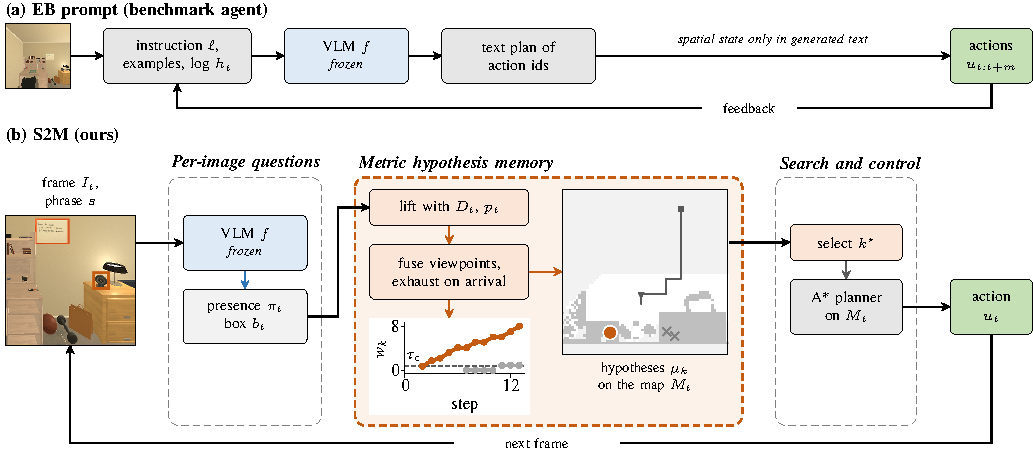
\includegraphics[width=\linewidth]{figures/fig_arch.pdf}
\caption[The benchmark's agent and the Semantic-to-Metric agent]{\textbf{(a)}~The EB prompt maps the image $I_t$,
the instruction $\ell$, and the history $h_t$ to a text plan $u_{t:t+m}$ with the VLM $f$. \textbf{(b)}~\ours asks
$f$ for the presence $\pi_t$ and box $b_t$ of the phrase $s$, lifts them with depth $D_t$ and pose $p_t$ into
hypotheses $\mu_k$ with evidence $w_k$, selects $k^\star$, and plans $u_t$ on the map $M_t$. Thumbnails: a
Long-horizon test episode, with the VLM's box on the target, the evidence of the target (orange) rising to ten times
the commit threshold $\tau_\mathrm{c}$ while two look-alikes (grey) stay near or below it, and the map with the path,
the target (orange), and the look-alikes ($\times$). Blue: the frozen VLM; orange: the hypothesis memory of \ours and
the selection that reads it.}
\label{fig:arch}
\end{figure}

The agent is evaluated on the full EB-Navigation test set and the full RoboTHOR validation split with two model
generations, repeated runs, and paired statistics. Changing the model's role moves it further than scaling it. With
Qwen3-VL-4B at 4-bit, \ours succeeds in \nSThree\% of the EB-Navigation test episodes, \nGainThree{} percentage points
more than the benchmark's agent with the same model, as much as the tenfold scale-up from InternVL3-8B to 78B gives,
and it closes \nGapClosed\% of the gap to the oracle planner. Each step takes \nSecS\,s instead of \nSecEB\,s, because
the model answers two short questions instead of writing a plan.

\section{Contributions}
\label{sec:intro-contrib}
The thesis makes the following contributions.
\begin{enumerate}
\item \textbf{A diagnosis of small-VLM navigators.} Controlled experiments on the same test episodes show that small
VLMs fail as navigation agents because they must keep spatial state in generated text, not because they cannot
recognize the target or plan a path. The diagnosis yields four predictions, all of which the experiments confirm.
\item \textbf{The VLM as a sensor, not a planner.} \ours inverts the control of MLLM agents: a metric controller asks
the VLM only questions that the current image can settle, and the VLM never sees the history, the map, or the plan.
\item \textbf{Evidence fusion for a generative sensor.} A metric hypothesis memory accumulates the model's presence
and box answers over distinct viewpoints and discards look-alikes on arrival, which turns unreliable single
answers into a stable target. A modular agent that is \ours without fusion and the crop check, and so acts on single-view
answers with the same model and planner, trails \ours by \nSOverMod{} percentage points.
\item \textbf{Navigation from RGB alone.} A per-frame ground-plane scale for monocular depth raises RGB-only success
from \nRGBGlobal\% with a global scale to \nRGBThree\%, within \nGapRGBAbs{} percentage points of a depth sensor.
\item \textbf{A training-free 4B agent that rivals far larger ones.} From RGB alone, \ours is above GPT-4o, both fine-tuned
4B agents, and \nNTrainFreeBelowRGB{} of \nNTrainFree{} training-free agents built on 8B to frontier-scale models; with a depth sensor, changing the
model's role gives as much as a tenfold larger model. With Qwen2.5-VL-3B~\cite{bai2025qwen25vl}
its gain over the benchmark's agent grows to \nGainTwo{} percentage points, and on RoboTHOR it reaches \nRoboSR\%
success, above ten published zero-shot methods.
\end{enumerate}

\section{Thesis organization}
\label{sec:intro-outline}
\Cref{chap:literature} reviews embodied navigation, zero-shot object navigation, MLLM agents, and the methods for
memory, verification, and geometry on which \ours builds. \Cref{chap:prelim} defines the task, the benchmarks, the
metrics, the models, and the statistical protocol. \Cref{chap:diagnosis} diagnoses why a small VLM fails when it is
prompted as the benchmark's agent and derives four predictions. \Cref{chap:method} presents \ours, and
\cref{chap:experiments} tests the predictions and analyses the agent. \Cref{chap:conclusions} answers the research
questions, discusses the findings and limitations, and outlines future work. \Cref{app:impl} lists the prompts,
parameters, and serving settings, and \cref{app:results} gives the evaluation protocol and additional results.


\chapter{Literature Review}
\label{chap:literature}
This chapter reviews the work on which the thesis builds and against which it is measured. It moves from the
navigation problem itself (\cref{sec:lit-nav,sec:lit-objnav}) to the use of foundation models as embodied agents
(\cref{sec:lit-agents}), and then to three ingredients of \ours: memory that attaches semantics to geometry
(\cref{sec:lit-memory}), verification and search with VLM queries (\cref{sec:lit-verify}), and geometry from images
(\cref{sec:lit-geometry}). \Cref{sec:lit-gap} states the gap that the thesis addresses.

\section{Embodied navigation}
\label{sec:lit-nav}
\subsection{Classical navigation}
Classical mobile robots separate mapping, localization, and planning. Occupancy grids represent free and occupied
space as a probabilistic grid built from range measurements~\cite{elfes1989occupancy}; frontier-based exploration
drives the robot to the boundary between known free space and unknown space until the map is complete~\cite{yamauchi1997frontier};
and graph search such as A*~\cite{hart1968astar} computes collision-free paths on the map. These components are
reliable, interpretable, and require no learning, and they form the geometric core of most modular navigation
systems~\cite{thrun2005probabilistic}. What they lack is semantics: a classical map records where the robot can go,
not where a ``kettle'' or ``something to sit on'' is.

\subsection{Benchmarks for embodied navigation}
Simulators of indoor scenes, such as AI2-THOR~\cite{kolve2017ai2thor} and Habitat~\cite{savva2019habitat}, made
large-scale evaluation of embodied agents possible. Anderson~\etal{} proposed the evaluation framework that most
benchmarks follow, including success weighted by path length (SPL)~\cite{anderson2018evaluation}. Object-goal
navigation (ObjectNav) asks the agent to reach an instance of a named category~\cite{batra2020objectnav};
RoboTHOR~\cite{deitke2020robothor} poses it in apartments built both in simulation and in the real world.
Vision-and-language navigation (VLN) asks the agent to follow route instructions~\cite{anderson2018vln}.
EmbodiedBench~\cite{yang2025embodiedbench} evaluates multimodal LLMs on high- and low-level embodied tasks through a
standardized action interface, and its EB-Navigation benchmark is the main testbed of this thesis. Related benchmarks
probe embodied decision making and navigation reasoning of language models~\cite{li2024embodied,qiao2025navbench}.

\subsection{Learned navigation policies}
End-to-end learning maps observations directly to actions. Policies trained for ObjectNav in large procedurally
generated houses reach strong results on RoboTHOR~\cite{deitke2022procthor}. Semantic exploration learns where a
category is likely to be and builds an explicit semantic map~\cite{chaplot2020object}. More recently,
vision-language-action models fine-tune a VLM to output navigation actions from video~\cite{zhang2024navid,cheng2024navila,wei2025streamvln},
and diffusion policies and world models generate trajectories or predict future views for planning~\cite{sridhar2023nomad,cai2025navdp,bar2024navigation}.
Learned policies capture regularities of indoor scenes that hand-written rules miss, such as where kitchens tend
to be. They pay for this with task-specific data, long training on large simulated datasets, and sensitivity to the
gap between the training scenes and the deployment scenes. \ours uses a frozen model without training and keeps the
navigation itself in classical geometry, which transfers without retraining.

\subsection{Compact vision-language models}
The VLMs that a robot can run locally are the small members of open model families. Qwen2.5-VL and Qwen3-VL provide
models of 3--8B parameters that answer questions about images and return bounding boxes for objects named in
text~\cite{bai2025qwen25vl,bai2025qwen3vl}. Weight quantization such as AWQ stores the weights in 4 bits with a small
loss in accuracy~\cite{lin2024awq}, and serving engines with paged attention run such models efficiently on a single
GPU~\cite{kwon2023vllm}. Together they make it possible to run a 4B model next to a simulator on one 8\,GB consumer
GPU, the setting of this thesis. On embodied benchmarks, however, these models lag far behind frontier models when
they are used as agents~\cite{yang2025embodiedbench}; the thesis asks whether this gap reflects their perception or
their role.

\section{Zero-shot object navigation}
\label{sec:lit-objnav}
Zero-shot ObjectNav removes task-specific training by combining an open-vocabulary perception model with a map and a
planner. CoW pairs open-vocabulary localization with frontier exploration~\cite{gadre2022cows}. Later systems add
semantic reasoning about where to search. ESC and L3MVN ask a language model which frontier is likely to lead to
the target~\cite{zhou2023esc,yu2023l3mvn}; VLFM builds a value map from vision-language similarity~\cite{yokoyama2023vlfm};
OpenFMNav and LGX use foundation models to propose and select goals~\cite{kuang2024openfmnav,dorbala2024lgx};
SG-Nav, MSGNav, and UniGoal reason over scene or goal graphs with an LLM~\cite{yin2024online,huang2025msgnav,yin2025unigoal};
WMNav uses a world model~\cite{nie2025wmnav}; CogNav models navigation as a cognitive state machine~\cite{cao2024cognav};
STRIVE queries a VLM over a structured representation~\cite{zhu2025strive}; and MVP-Nav and ForesightNav plan over
multi-layer value maps and semantic-geometric predictions~\cite{xie2026mvpnav,liu2026foresightnav}.
Instruction-following agents extend this structure from categories to free-form instructions by grounding
language in maps and scene graphs~\cite{long2024instructnav,rana2023sayplan,werby2024hierarchical,huang2023vlmaps,shah2022lmnav}.

These systems share the modular structure of \ours: perception produces detections, a map stores them, and a
planner acts. They differ from \ours in three respects. First, most use dedicated open-vocabulary detectors such as
OWL-ViT or Grounding DINO~\cite{minderer2022owlvit,liu2024groundingdino}, often together with a large language model
for reasoning; \ours uses one small generative VLM as its only perception model, which reads open instructions
directly. Second, many ask a language model where to explore; \ours never asks the model where to go, and its
exploration follows geometric rules. Third, a detector returns calibrated scores for a fixed vocabulary, whereas a
generative VLM writes its boxes as text and places boxes in views that do not show the target
(\cref{sec:diag-probe}). The memory of \ours is designed for this error profile.

\section{Multimodal LLMs as embodied agents}
\label{sec:lit-agents}
A second line of work uses a multimodal LLM as the whole agent. SayCan grounds an LLM's plans in the affordances
of learned skills~\cite{ahn2022saycan}. In EmbodiedBench, the model maps the image, the instruction, and the text
history directly to a plan of actions~\cite{yang2025embodiedbench}. Agents are improved by embodied pre-training,
online reinforcement learning, or policy-level reasoning~\cite{chen2025transforming,wang2025vagen,zhang2025embodiedx,liu2025robogpt},
or at test time with reflection, experience, workflow memory, multi-memory architectures, and
verifiers~\cite{shinn2023reflexion,zhao2023expel,chen2024automanual,wang2024agent,lei2025robomemory,singhi2026think}.

On EB-Navigation specifically, training-free agents add a scene graph~\cite{huang2025esca}, a module graph~\cite{wang2026mosaic},
a skill library~\cite{ju2026embodiskill}, brain-inspired memory~\cite{ma2026brainmem},
an optimized harness~\cite{lee2026emho}, self-evolution~\cite{liang2026robofoundry}, or a library of perception and
mapping tools~\cite{zhou2026enabling}, and SeeNav-Agent renders the target into a bird's-eye view~\cite{wang2025seenav}.
Fine-tuned agents train world models or a Q-model around a 4B policy~\cite{jang2026musix,xie2026sva}.
All of these agents keep the model as the planner and as the reader of its own memory. Whatever is added, a
scene graph, a skill, or a tool output, enters the model's context as text or as an image, and the model must
interpret it and decide. This places the hardest part of the task, integrating observations over time into a
decision, on the model. The reported gains therefore grow with model size: the training-free agents on
EB-Navigation use models of 8B parameters up to frontier scale, and the agents that work with 4B models require
training. \ours takes the opposite position: the VLM is only a sensor, and its answers feed an explicit metric
estimator and planner.

\Cref{tab:lit-compare} contrasts the main families of approaches along the dimensions that matter for this thesis.

\begin{table}[htbp]
\centering\small
\caption[Families of approaches to instruction-following navigation]{Families of approaches to instruction-following
navigation. ``Open'' instructions describe the target by use or appearance as well as by name.}
\label{tab:lit-compare}
\resizebox{\linewidth}{!}{%
\begin{tabular}{@{}lllllc@{}}
\toprule
Family & Who decides & Perception & Spatial state & Training & Open instructions\\
\midrule
Prompted MLLM agent~\cite{yang2025embodiedbench} & the model & the model & text history & none & yes\\
Training-free MLLM agents~\cite{lee2026emho,ma2026brainmem,zhou2026enabling} & the model & model, tools & text, graphs, tool state & none & yes\\
Fine-tuned VLM agents~\cite{xie2026sva,jang2026musix} & the model & the model & learned & task-specific & yes\\
Modular zero-shot ObjectNav~\cite{gadre2022cows,yokoyama2023vlfm,yin2024online} & map, planner, often an LLM & detector & metric map & none & mostly categories\\
Learned ObjectNav policies~\cite{deitke2022procthor,chaplot2020object} & the policy & learned & learned or map & task-specific & categories\\
\midrule
\ours (this thesis) & metric controller & one small VLM & metric hypotheses, map & none & yes\\
\bottomrule
\end{tabular}}
\end{table}

\section{Semantic memory for embodied agents}
\label{sec:lit-memory}
Embodied agents attach semantics to geometry in many forms: open-vocabulary 3D scene graphs~\cite{gu2023conceptgraphs},
online semantic maps for changing scenes~\cite{jiang2025dualmap}, language fields and semantic Gaussian
splatting~\cite{katragadda2025online,lee2026embodiedsplat}, and long-horizon spatio-temporal memories for exploration,
question answering, and navigation~\cite{yang2024scene,anwar2024remembr,ginting2025enter}. These representations
are rich and general. They are built with dedicated encoders or large models, and they store far more than a
navigation agent needs to reach one object: a full scene graph or language field must be constructed and queried
at every step, which is costly on a small GPU and adds failure modes of its own. A navigation agent needs to know
where the target might be, how much evidence supports each candidate, and where it can move.

The memory of \ours also has a classical ancestor outside semantic mapping. Multiple-hypothesis
tracking keeps several candidate explanations of noisy, possibly false detections, associates each new detection
with one of them, and lets the evidence decide~\cite{reid1979algorithm}; probabilistic robotics applies the same
idea to localization and mapping~\cite{thrun2005probabilistic}. Active visual object search plans where a robot should
look for an object, using probabilistic models of where objects tend to be and how reliable its detector
is~\cite{aydemir2011search,aydemir2013active}. \ours borrows the hypothesis bookkeeping of tracking and the
detector-aware search of active object search, and replaces the trained detector of both with the yes/no and box
answers of a generative VLM, whose errors (confident boxes on look-alikes, repeated answers from one view) shape how
the evidence is counted.

Closest to the memory of \ours are two object-navigation systems. ApexNav fuses target-centric detections over time
to suppress false positives~\cite{zhang2025apexnav}, and AECNav treats expected but absent detections as negative
evidence~\cite{liu2026aecnav}. \ours shares both ideas and applies them at the minimal end of the spectrum: its memory
is a short list of metric target hypotheses whose evidence grows only with distinct viewpoints, a choice that
matters for a generative sensor whose repeated answers from the same view are not independent.

\section{Verification, uncertainty, and search}
\label{sec:lit-verify}
Spatially explicit prompting, such as marking candidate regions or actions in the image, improves the spatial
decisions of VLMs~\cite{yang2023mark,nasiriany2024pivot,goetting2024navigation}. Test-time sampling and verification,
adaptive allocation of test-time compute, and uncertainty-conditioned execution improve vision-language-action
models and embodied planners~\cite{kwok2025robomonkey,dao2026direct,choi2026scale}, and calibrated uncertainty lets
robots ask for help or explore until confident~\cite{ren2023robots,liang2024introspective,ren2024explore}.
These methods share one insight with \ours: a model's answer is more useful when the agent knows how much to
trust it. They differ in where the trust comes from. Sampling and verification spend more model calls on the same
decision; calibrated uncertainty asks the model how sure it is. \ours obtains trust from geometry: an answer gains
weight when the same location is confirmed from a different viewpoint, and a candidate is ruled out once the agent
reaches it without ending the task. It spends an extra query, a magnified crop, only where the evidence is weak.

\section{Geometry from images}
\label{sec:lit-geometry}
Learned reconstruction and depth networks recover metric geometry from RGB images: feed-forward reconstruction and
dense SLAM with learned priors~\cite{wang2025vggt,murai2024mast,maggio2025vggt}, zero-shot stereo~\cite{wen2025foundationstereo},
and monocular metric depth~\cite{yang2024depthv2,lin2025depth}. Sensor choices can change the conclusions of embodied
evaluations~\cite{corlito2026sensor,wang2025rethinking}, so an agent that claims to work from RGB must be evaluated
without privileged depth or pose. Monocular visual odometry fixes its unknown scale from the ground plane and the
known camera height~\cite{song2014robust}; \ours applies the same constraint to every frame of a monocular metric
depth network. Concurrently with this work, Li~\etal{} run Qwen3-VL-4B zero-shot and accumulate its answers as
per-direction scores in a bird's-eye field for vision-language navigation~\cite{li2026structure}; \ours instead lifts
boxes to metric target hypotheses for object navigation.

\section{Summary and research gap}
\label{sec:lit-gap}
Two lines of work meet in this thesis. MLLM agents follow open instructions but keep the model in charge of the plan,
and their gains depend on large models or training. Modular object-navigation systems keep a metric map and a
planner but rely on dedicated detectors, fixed vocabularies, and often large language models for exploration. No
existing agent lets a small generative VLM drive open-instruction navigation, and no study has isolated why such a
model fails when it is used as the agent. The thesis addresses both gaps: it diagnoses the failure
(\cref{chap:diagnosis}) and builds an agent in which the small VLM is only a semantic sensor (\cref{chap:method}).


\chapter{Preliminaries}
\label{chap:prelim}
This chapter fixes the notation and the experimental ground on which the rest of the thesis stands: the navigation
task (\cref{sec:pre-task}), the two benchmarks (\cref{sec:pre-bench}), the metrics (\cref{sec:pre-metrics}), the
models and their deployment (\cref{sec:pre-models}), and the protocol and statistics used for every comparison
(\cref{sec:pre-protocol}).

\section{Task definition}
\label{sec:pre-task}
An episode gives an instruction $\ell$ that identifies one object with floor position $x^\star\in\mathbb{R}^2$. At
step $t$ the agent observes an RGB frame $I_t$, a depth image $D_t$, a pose $p_t=(x_t,\theta_t,\phi_t)$ consisting of
floor position, heading, and camera tilt, and the success flag $o_{t-1}$ of its last action. It chooses an action
$u_t\in\mathcal{U}$, where $\mathcal{U}$ contains four 0.25\,m translations (forward, backward, left, right), two
90$^\circ$ turns, and two 30$^\circ$ camera tilts. The episode is successful if
\begin{equation}
\exists\, t\le T:\ \lVert x_t-x^\star\rVert\le 1\,\text{m},\qquad T=20 .
\label{eq:success}
\end{equation}
A rejected action, for instance a translation into furniture, leaves the pose unchanged and sets $o_t=0$. The agent
never observes $x^\star$; it observes only the instruction and its own sensors.

\Cref{tab:notation} collects the symbols used in the rest of the thesis.

\begin{table}[htbp]
\centering\small
\caption{Notation.}
\label{tab:notation}
\begin{tabular*}{\linewidth}{@{\extracolsep{\fill}}ll@{}}
\toprule
Symbol & Meaning\\
\midrule
$\ell$, $s$ & instruction; target phrase extracted from it\\
$I_t$, $D_t$, $p_t$ & RGB frame, depth image, and pose $(x_t,\theta_t,\phi_t)$ at step $t$\\
$u_t$, $o_t$ & action and its success flag\\
$f$ & the frozen VLM\\
$\pi_t$, $b_t$ & presence probability and box returned by $f$ for $s$ on $I_t$\\
$a_t$ & weight of the observation of step $t$\\
$q_t$ & floor point to which a box is lifted\\
$\mu_k$, $w_k$, $V_k$ & position, evidence, and viewing poses of hypothesis $k$\\
$M_t$ & occupancy map\\
$\mathcal{B}_t$ & belief, the hypotheses together with the map\\
$\tau_\mathrm{c}$, $\tau_\mathrm{keep}$ & commit and keep thresholds\\
\bottomrule
\end{tabular*}
\end{table}

\section{Benchmarks}
\label{sec:pre-bench}
\subsection{EB-Navigation}
EB-Navigation~\cite{yang2025embodiedbench} poses the task of \cref{sec:pre-task} in single AI2-THOR
rooms~\cite{kolve2017ai2thor}. Its test set has 300 episodes in five subsets of 60, which differ only in how the
target is described or where the agent starts.
\begin{description}
\item[Base] names the target category, e.g.\ ``navigate to the AlarmClock in the room''.
\item[Common] describes the object by its use or by common sense instead of its name.
\item[Complex] embeds the target in a longer instruction with irrelevant context.
\item[Visual] describes only the appearance of the object: colour, shape, or material.
\item[Long] repeats Base with the agent turned away from the target, so the target starts behind the agent.
\end{description}
\Cref{tab:subsets} shows the five instructions of one test scene, FloorPlan13, in which the target is a toaster. The
same object is named directly, described by its use, buried in an unrelated description of the room, described only
by its colour and shape, and named again with the agent facing away from it.

\begin{table}[htbp]
\centering\small
\caption[The five EB-Navigation subsets]{The five EB-Navigation subsets, illustrated by the test instructions of
scene FloorPlan13 (target: a toaster).}
\label{tab:subsets}
\begin{tabular}{@{}lp{0.74\linewidth}@{}}
\toprule
Subset & Instruction\\
\midrule
Base & ``navigate to the Toaster in the room and be as close as possible to it''\\
Common & ``I'd like a machine that could toast some slices of bread until they are crisp. Can you navigate to that
object and stay close?''\\
Complex & ``The room is filled with the golden glow of the late afternoon sun, making it feel warm and inviting.
There's a fruit basket nearby, with bananas and apples spilling out. Please move towards the toaster. Everything feels
so peaceful right now.''\\
Visual & ``Approach the red rectangular item with black edges around the sides.''\\
Long & ``navigate to the Toaster in the room and be as close as possible to it'' (start heading rotated by
180$^\circ$)\\
\bottomrule
\end{tabular}
\end{table}

The benchmark ends an episode as soon as the agent is within 1\,m of the target, so on EB-Navigation an agent never
has to decide when to stop. All experiments use the official environment, action set, and success test. The camera
renders $500{\times}500$ RGB and depth images with a 100$^\circ$ field of view at 1.576\,m above the floor, and the
agent body is modelled as a disc of 0.2\,m radius. Translations snap to the simulator's grid, so a 0.25\,m move may
end up to a few centimetres away from its nominal position.

\subsection{RoboTHOR ObjectNav}
RoboTHOR~\cite{deitke2020robothor} poses object-goal navigation in apartments with several rooms. The validation
split used here has \nRoboN{} episodes in 15 apartments with 12 target categories. The agent uses LoCoBot actuation
with stochastic motion, 30$^\circ$ turns, and at most 500 steps. Unlike EB-Navigation, it must issue a Stop action;
an episode succeeds only if Stop is issued within 1\,m of a visible object of the target category. RoboTHOR therefore
tests two things that EB-Navigation does not: larger scenes and an explicit stop decision. Its camera renders
$640{\times}480$ images with a 63.5$^\circ$ field of view, which shows less of the room per frame than the wide
camera of EB-Navigation. \Cref{tab:bench-compare} summarizes the differences between the two benchmarks.

\begin{table}[htbp]
\centering\small
\caption{The two benchmarks.}
\label{tab:bench-compare}
\begin{tabular*}{\linewidth}{@{\extracolsep{\fill}}lll@{}}
\toprule
 & EB-Navigation & RoboTHOR ObjectNav\\
\midrule
Scenes & single iTHOR rooms & 15 multi-room apartments\\
Episodes evaluated & 300 (test) & \nRoboN{} (validation)\\
Goal description & five instruction types & 12 object categories\\
Step budget & 20 & 500\\
Translations & 0.25\,m, four directions & 0.25\,m forward, stochastic\\
Turns, tilts & 90$^\circ$, 30$^\circ$ & 30$^\circ$, 30$^\circ$\\
Camera & $500{\times}500$, 100$^\circ$ & $640{\times}480$, 63.5$^\circ$\\
End of episode & automatic on success & agent issues Stop\\
Metrics & SR & SR, SPL\\
\bottomrule
\end{tabular*}
\end{table}

\section{Evaluation metrics}
\label{sec:pre-metrics}
The main metric is the \emph{success rate} (SR), the fraction of episodes that satisfy the success condition. On
RoboTHOR, \emph{success weighted by path length} (SPL)~\cite{anderson2018evaluation} additionally rewards short paths,
\begin{equation}
\mathrm{SPL}=\frac{1}{N}\sum_{i=1}^{N} S_i\,\frac{L_i^\star}{\max(L_i,L_i^\star)},
\label{eq:spl}
\end{equation}
where $S_i$ is the success indicator of episode $i$, $L_i$ the length of the agent's path, and $L_i^\star$ the
length of the shortest path to the target. On EB-Navigation the thesis also reports the number of steps to success,
success within a step budget, and the number of VLM calls and tokens per episode.

To explain failures, each failed EB-Navigation episode is assigned the first matching outcome of a fixed taxonomy:
the target never enters the view (\emph{never seen}); the final distance is at most 1.5\,m (\emph{near miss}); the
target is out of view in the last five steps (\emph{lost after seen}); at least 30\% of the actions are rejected
(\emph{blocked}); at least three immediate reversals (\emph{oscillation}); otherwise \emph{approach failure}.
Visibility comes from the simulator's object metadata, which is used for analysis only and never given to an agent.

\section{Models and deployment}
\label{sec:pre-models}
Two open VLMs of different generations serve as the agent's model: Qwen3-VL-4B-Instruct~\cite{bai2025qwen3vl} and
Qwen2.5-VL-3B-Instruct~\cite{bai2025qwen25vl}. Both are served locally with vLLM~\cite{kwon2023vllm} at temperature 0
on one consumer GPU with 8\,GB of memory (an NVIDIA RTX~5060), which also renders the simulator. \ours uses the 4-bit
AWQ checkpoints of both models~\cite{lin2024awq}. Monocular depth for the RGB-only configuration comes from Depth
Anything V2 Metric-Indoor-Base~\cite{yang2024depthv2}, which runs on the CPU. No model is fine-tuned at any point. \Cref{tab:system} lists the hardware and software. The GPU is shared by the
VLM server and the simulator's renderer, so the model server is limited to a fraction of the 8\,GB of GPU memory.

\begin{table}[htbp]
\centering\small
\caption{Hardware and software used for all experiments.}
\label{tab:system}
\begin{tabular}{@{}lp{0.68\linewidth}@{}}
\toprule
Component & Setting\\
\midrule
GPU & one NVIDIA GeForce RTX 5060, 8\,GB, shared by the VLM server and the renderer\\
CPU and memory & 28 hardware threads, 32\,GB RAM\\
Operating system & Ubuntu 20.04\\
Simulator & AI2-THOR 5.0 with cloud rendering\\
VLM serving & vLLM 0.32, temperature 0, 4-bit AWQ weights for \ours\\
Models & Qwen3-VL-4B-Instruct, Qwen2.5-VL-3B-Instruct\\
Monocular depth & Depth Anything V2 Metric-Indoor-Base, on the CPU\\
\bottomrule
\end{tabular}
\end{table}

\section{Protocol and statistics}
\label{sec:pre-protocol}
\subsection{Development and test splits}
All design choices and parameters of \ours were selected on a separate development split and frozen before its
test runs. EmbodiedBench provides targets and instruction variants for 90 iTHOR rooms, and its test set uses 60
of them. Rerunning the benchmark's own generator on the other 30 rooms gives 150 development targets in five subsets of
30; three generator seeds give each target three start poses, 450 development episodes in all (\cref{sec:appB-dev}). Test results are reported only on the complete official splits.

For the Qwen3-VL-2B EB-prompt baseline, frequent unparseable outputs led us to stop an incomplete test run.
Before the final test comparison, we fixed a rule to select the official or a length-bounded output schema using
150 development episodes; the bounded schema was selected and the partial test run discarded. The EB baseline
uses FP8 weights, while \ours uses 4-bit AWQ weights.

\subsection{Statistical tests}
All agents run on the same 300 test episodes, so each comparison uses per-episode differences. \ours was run three
times on the EB-Navigation test set and the RGB-only configuration twice; a configuration run several times enters
with its per-episode mean success. Confidence intervals are percentile intervals of $10^4$ episode-level bootstrap
resamples~\cite{efron1993bootstrap}. $p$-values are two-sided sign-flip permutation tests with $10^6$ random sign
assignments. The seven ablation variants of \cref{sec:exp-ablation} are corrected together with the Holm
procedure~\cite{holm1979simple}, and comparisons of two single binary runs use the exact McNemar
test~\cite{mcnemar1947note}.

\subsection{Why paired tests}
All agents are evaluated on the same 300 episodes, and episodes differ greatly in difficulty: a target in plain
view at the start is solved by almost every agent, while a small target behind furniture is solved by few. An
unpaired comparison of two success rates treats this variation as noise and needs large differences to reach
significance. A paired comparison removes it: for each episode it takes the difference between the two agents'
outcomes, so only episodes on which the agents disagree carry information. The bootstrap resamples these
per-episode differences, and the sign-flip test asks how often a random assignment of signs to them produces a mean
difference as large as the observed one. When one agent was run several times, its per-episode mean success
enters the comparison, which uses all runs without counting the same episode twice. The Holm procedure controls the
probability of any false positive among the seven ablation variants at 5\%, which is stricter than testing each
variant on its own.

\section{Summary}
This chapter defined a navigation task with a 20-step budget and eight discrete actions, two benchmarks that test it
in single rooms and in apartments with an explicit stop, and a protocol in which every comparison is paired over the
same episodes and every parameter is fixed on a separate development split. The next chapter uses this setting to
diagnose why a small VLM fails when it is prompted as the agent.


\chapter{Why Small VLMs Fail as Navigation Agents}
\label{chap:diagnosis}
This chapter answers the first research question: why does a small VLM fail when it is used as a navigation agent?
It describes the benchmark's prompted agent (\cref{sec:diag-eb}), recasts its decision as a factorization that
separates perception from state (\cref{sec:diag-factor}), and then tests the three candidate causes in turn: motion
planning (\cref{sec:diag-oracle}), recognition (\cref{sec:diag-probe}), and the keeping of spatial state
(\cref{sec:diag-state}). \Cref{sec:diag-predictions} turns the diagnosis into four predictions.

\section{The prompted agent}
\label{sec:diag-eb}
The benchmark's own agent, which this thesis calls the \emph{EB prompt}, maps the image and its text history
$h_t=(u_{0:t-1},o_{0:t-1})$ directly to a plan,
\begin{equation}
(u_t,\dots,u_{t+m})=f(I_t,\ell,h_t),
\label{eq:ebpolicy}
\end{equation}
which is executed until an action fails. The prompt contains the instruction, the action list, three worked
examples, and the history, and the model must reply in a JSON format with a description of the visual state, its
reasoning, a language plan, and the action identifiers. All spatial state, namely where the target was, what the room
contains, and how the agent has turned, must be carried by $h_t$ and the generated reasoning. The thesis uses the
benchmark's prompts, examples, parser, and plan execution unchanged. With Qwen3-VL-4B, \nEBThreeParse.

\section{A factorization of the decision}
\label{sec:diag-factor}
The same decision can be factorized so that the model answers only questions about the current image and all state
lives outside it:
\begin{equation}
\begin{gathered}
(\pi_t,b_t)=f(I_t,s),\\
\mathcal{B}_t=g(\mathcal{B}_{t-1},\pi_t,b_t,D_t,p_t),\qquad u_t=\rho(\mathcal{B}_t,p_t),
\end{gathered}
\label{eq:factor}
\end{equation}
where $s$ is a target phrase, $\pi_t$ and $b_t$ are the presence probability and box of $s$ in $I_t$, the update $g$
maintains a metric belief $\mathcal{B}_t$, and the policy $\rho$ chooses the action from the belief alone.
\Cref{eq:ebpolicy,eq:factor} use the same model, the same observations, and the same actions. They differ only in
the role of the model: in \cref{eq:ebpolicy} it keeps the state and makes every decision, in \cref{eq:factor} it
answers two questions that the current image can settle. This factorization is the basis of \ours
(\cref{chap:method}) and of the controlled experiments below, which replace one part of it at a time.

\section{Planning is not the bottleneck}
\label{sec:diag-oracle}
If the factorized agent is given the true target position $x^\star$ in place of its belief about the target, with
the same occupancy map and planner, it solves \nOracle\% of the 300 test episodes: \nOracleBase\% on each of the first
four subsets and \nOracleLong\% on Long, where the agent must first turn around. The remaining failures come from the
20-step budget and from targets that cannot be approached within 1\,m. Motion planning in these rooms is therefore
nearly solved by classical geometry, and the oracle serves as the upper bound in all later comparisons.

\section{Single views are informative but unreliable}
\label{sec:diag-probe}
To measure recognition in isolation, the start view of each test episode in the first four subsets and the three
other 90$^\circ$ headings are rendered, and the VLM is queried with the target phrase $s$ on each view. A box counts
as correct if its intersection-over-union with the target's ground-truth box is at least 0.3.

Qwen3-VL-4B places a correct box on the visible target in \nProbeThreeBase, \nProbeThreeCommon, \nProbeThreeComplex,
and \nProbeThreeVisual\% of the views on Base, Common, Complex, and Visual, from 75 visible instances per subset.
Qwen2.5-VL-3B does so in \nProbeTwoBase, \nProbeTwoCommon, \nProbeTwoComplex, and \nProbeTwoVisual\%. Recognition is
therefore usable whenever the instruction names or implies a category, and weakest when it describes only appearance.

The model also errs in the other direction. On views that do not show the target, Qwen3-VL-4B still places a box in
\nFalseBoxNamedLo--\nFalseBoxNamedHi\% of the cases for named categories and in \nFalseBoxVisual\% for appearance-only
phrases. \Cref{tab:probe,fig:probe} give both rates for both models. The two models make different trade-offs.
Qwen3-VL-4B finds the target about twice as often as Qwen2.5-VL-3B, but it also places more boxes on views that do
not show the target, most of all for appearance-only phrases. Qwen2.5-VL-3B answers more conservatively and misses
more targets. Neither model is reliable enough to act on one answer: the first would follow look-alikes, the second
would walk past targets. A single answer is therefore evidence, not a decision.

\begin{figure}[htbp]
\centering
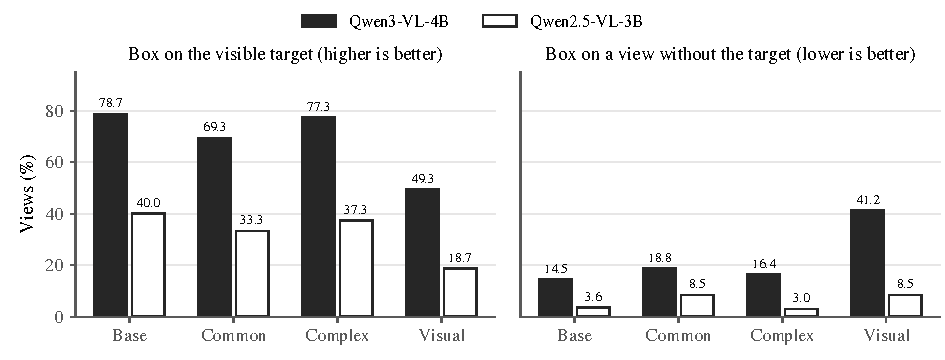
\includegraphics[width=\linewidth]{figures/th_probe.pdf}
\caption[Recognition from single views]{Recognition from single views (\cref{tab:probe}). Left: views showing the
target in which the model places a box with IoU${\ge}0.3$ on it. Right: views without the target in which the model
still places a box.}
\label{fig:probe}
\end{figure}
An agent that acts on every box would be drawn to look-alikes; an agent that ignores weak boxes would miss real
targets. This observation motivates the evidence accumulation of \cref{sec:method-memory}.

\begin{table}[htbp]
\centering\small
\caption[Single-view probe]{Single-view probe on the test episodes of the first four subsets (start view and the
three other 90$^\circ$ headings; 75 views with the target visible per subset).}
\label{tab:probe}
\begin{tabular*}{\linewidth}{@{\extracolsep{\fill}}lcccccccc@{}}
\toprule
& \multicolumn{4}{c}{Box on the target, IoU${\ge}0.3$ (\%)} & \multicolumn{4}{c}{Box on a view without it (\%)}\\
\cmidrule(lr){2-5}\cmidrule(l){6-9}
Model & Base & Common & Complex & Visual & Base & Common & Complex & Visual\\
\midrule
Qwen3-VL-4B & 78.7 & 69.3 & 77.3 & 49.3 & 14.5 & 18.8 & 16.4 & 41.2\\
Qwen2.5-VL-3B & 40.0 & 33.3 & 37.3 & 18.7 & 3.6 & 8.5 & 3.0 & 8.5\\
\bottomrule
\end{tabular*}

\end{table}

\section{The prompted agent loses spatial state}
\label{sec:diag-state}
If neither planning nor recognition explains the failure, the remaining candidate is the keeping of spatial state.
The failure taxonomy of \cref{sec:pre-metrics} tests this directly. Of the \nFailEBThree{} episodes that the EB prompt
fails with Qwen3-VL-4B, \nLostEBThree{} lose a target that was in view, \nBlockedEBThree{} are blocked by collisions,
and \nNearEBThree{} end within 1.5\,m of the target. In \nNeverLongEBThree{} Long episodes the agent never brings the
target into view at all.

The same pattern holds for the smaller model. With Qwen2.5-VL-3B the EB prompt loses a target it has seen in
\nLostEBTwo{} of the 300 episodes, more than with Qwen3-VL-4B, which shows that the problem grows as the model shrinks
(\cref{tab:taxonomy}).

Each of these failure modes is a failure of state. A target that was in view and is lost shows that the agent did not
remember where it was. Repeated collisions show that the agent did not remember which moves were rejected or where
the furniture is. A target behind the agent that is never seen shows that the agent did not keep track of which
directions it had already looked in. In every case the information was available to the agent at some step, and
in every case it had to be carried forward as generated text, which the model neither verifies against the image
nor updates consistently.

\subsection{An episode in detail}
\Cref{tab:eb-excerpt} follows the EB prompt with Qwen3-VL-4B through the first plans of one Long-horizon test
episode, in which the target is a pot and the agent starts facing away from it. At the first two steps the model
writes that the pot is on the counter to its right, although the simulator shows that the pot is not in view. It
plans moves toward this imagined pot, the moves run into the counter, and the model keeps planning the same moves.
Over the episode \tExcerptRejected{} of \tExcerptSteps{} actions are rejected and the pot is \tExcerptSeen{} seen. With
the same model on the same episode, \ours turns, finds the pot, and \tExcerptSOk{} in \tExcerptSSteps{} steps.

\begin{table}[htbp]
\centering\small
\caption[The EB prompt on one Long-horizon episode]{The first four plans of the EB prompt (Qwen3-VL-4B) on a
Long-horizon test episode whose target is a pot. ``Target in view'' comes from the simulator and is not available to
the agent; the last column counts the accepted and rejected actions of each plan.}
\label{tab:eb-excerpt}
\begin{tabular}{@{}rp{0.42\linewidth}cp{0.17\linewidth}c@{}}
\toprule
Step & Model's description of the view & In view & Plan & Acc./rej.\\
\midrule
0 & \textit{``The Pot is located on the countertop to the right side of the kitchen, near the stove.''} & no & right & 1 / 0\\
1 & \textit{``The Pot is located on the countertop to the right side of the kitchen, near the stove.''} & no & forward, forward, forward & 2 / 1\\
4 & \textit{``The current view shows a kitchen area with wooden cabinets on both sides.''} & no & right, forward, forward & 0 / 1\\
5 & \textit{``The current view shows a kitchen area with wooden cabinets on both sides.''} & no & right, forward, forward & 0 / 1\\
\bottomrule
\end{tabular}

\end{table}

The excerpt shows the mechanism of the failure. The model's description of the view is a belief, not an observation,
and nothing in the agent compares this belief with the image. Once written, the belief is carried into the next
prompt as part of the history and shapes the next plan. The rejected moves are recorded in the history as well, but
the model does not connect them with a wrong belief about where the target is.

\subsection{Why text is a poor carrier of spatial state}
Three properties of generated text explain why a small model cannot use it to keep spatial state.
\begin{enumerate}
\item \textbf{No grounding.} A sentence such as ``the pot is to my right'' has no coordinates. After the agent
turns, the sentence is no longer true, and the model must rewrite it from memory of the turn.
\item \textbf{No accumulation.} Text records one belief at a time. It has no natural way to express that a location
was confirmed from three viewpoints and contradicted from one, so evidence does not add up.
\item \textbf{No check.} The model generates the next belief conditioned on its previous one. A wrong belief is
therefore more likely to be repeated than corrected, as in \cref{tab:eb-excerpt}.
\end{enumerate}
A metric representation has the opposite properties: a position stays valid when the agent turns, evidence can be
added and subtracted, and every new frame can be compared with every stored hypothesis.

\section{Four testable predictions}
\label{sec:diag-predictions}
The diagnosis can be wrong, so it is stated as predictions that the experiments of \cref{chap:experiments} can
falsify. If small VLMs fail because their role makes them carry spatial state through text, an agent that keeps this
state outside the model, with the same model and the same actions, should
\begin{enumerate}[label=(\roman*)]
\item remove the never-seen and blocked failures and reduce the lost-after-seen ones;
\item gain most on Long, where the target must be remembered across turns;
\item gain least on Visual, where single-view recognition is weakest and remains the limit; and
\item depend far less on the size of the model, which no longer plans.
\end{enumerate}

\section{Summary}
\Cref{tab:diagnosis-summary} summarizes the diagnosis. Planning and recognition are adequate for the task; the
keeping of spatial state is not. The next chapter builds an agent that removes this burden from the model.

\begin{table}[htbp]
\centering\small
\caption{Summary of the diagnosis with Qwen3-VL-4B on the EB-Navigation test set.}
\label{tab:diagnosis-summary}
\begin{tabular}{@{}p{0.27\linewidth}p{0.36\linewidth}p{0.29\linewidth}@{}}
\toprule
Candidate cause & Evidence & Verdict\\
\midrule
Motion planning & oracle target: \nOracle\% success & not the bottleneck\\
Recognition & correct box on \nProbeThreeCommon--\nProbeThreeBase\% of visible named targets; false boxes on
\nFalseBoxNamedLo--\nFalseBoxNamedHi\% of empty views & usable, but unreliable alone\\
Spatial state & \nLostEBThree{} lost after seen, \nBlockedEBThree{} blocked, \nNeverLongEBThree{} Long never seen &
the bottleneck\\
\bottomrule
\end{tabular}
\end{table}


\chapter{The Semantic-to-Metric Agent}
\label{chap:method}
This chapter answers the second research question by presenting the Semantic-to-Metric agent. \ours instantiates the
factorization of \cref{eq:factor}: the VLM is its semantic sensor, and the agent owns all state and every decision.
\Cref{sec:method-principles} states the design principles, \cref{sec:method-overview} gives the complete loop, and
the following sections describe its parts in the order in which one step runs: the per-image questions
(\cref{sec:method-questions}), the metric hypothesis memory (\cref{sec:method-memory}), and search and control
(\cref{sec:method-control}). \Cref{sec:method-rgb,sec:method-stop} describe the RGB-only and explicit-stop variants.

\section{Design principles}
\label{sec:method-principles}
Three principles follow from the diagnosis of \cref{chap:diagnosis}.
\begin{enumerate}
\item \textbf{Ask only what the image can settle.} Every query to the VLM concerns the current frame, or a crop or tile
of it, and the target phrase. No query contains the action history, the map, or earlier answers, so every answer can
be checked against the image alone.
\item \textbf{Keep the state in metric form.} Where the target may be, which space is free, and which directions have
been looked at are stored as positions, evidence values, and grid cells, and are updated by explicit rules.
\item \textbf{Treat answers as evidence.} Because single answers are unreliable (\cref{sec:diag-probe}), no single
box decides the target. Evidence accumulates over distinct viewpoints and is withdrawn when an expected detection
does not appear.
\end{enumerate}
\Cref{tab:design-map} maps each part of \ours to the failure mode of \cref{sec:diag-state} that it addresses.

\begin{table}[htbp]
\centering\small
\caption{Parts of \ours and the diagnosed failure modes they address.}
\label{tab:design-map}
\begin{tabular*}{\linewidth}{@{\extracolsep{\fill}}lll@{}}
\toprule
Part & Section & Failure mode addressed\\
\midrule
Hypothesis memory with fusion & \cref{sec:method-memory} & lost after seen; acting on false boxes\\
Occupancy map and A* planner & \cref{sec:method-planning} & blocked by collisions\\
Look-around and exploration & \cref{sec:method-search} & target never seen (Long)\\
Crop check and tiled search & \cref{sec:method-questions} & weak or missed detections\\
Exhaustion on arrival & \cref{sec:method-commit} & committing to a look-alike\\
\bottomrule
\end{tabular*}
\end{table}

\section{Overview}
\label{sec:method-overview}
The belief $\mathcal{B}_t=(\mathcal{H}_t,M_t)$ of \ours consists of a list of target hypotheses $\mathcal{H}_t$ and an
occupancy map $M_t$. \Cref{fig:mech} shows one step as a flowchart, and \cref{alg:s2m} gives it as pseudocode.

\begin{figure}[htbp]
\centering
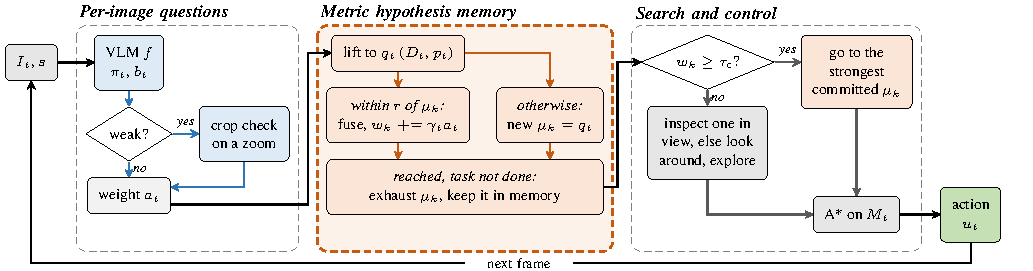
\includegraphics[width=\linewidth]{figures/fig_mech.pdf}
\caption[One step of \ours]{One step of \ours. The frozen VLM $f$ gives the presence $\pi_t$ and box $b_t$ of the
phrase $s$ on the frame $I_t$; a weak answer is checked on a crop or on tiles, which sets its weight $a_t$. The box is
lifted to a floor point $q_t$ with depth $D_t$ and pose $p_t$ and fused into a hypothesis $\mu_k$ within $r$, or
starts one; $\gamma_t<1$ discounts a repeated view, and a hypothesis that should be seen but is not loses $\lambda$ of
its evidence $w_k$. Above $\tau_c$ a hypothesis is committed, and the agent goes to $\mu_{k^\star}$; A* on the map
$M_t$ gives the action $u_t$.}
\label{fig:mech}
\end{figure}

\begin{algorithm}[htbp]
\caption{One step of \ours}
\label{alg:s2m}
\KwIn{frame $I_t$, depth $D_t$, pose $p_t$, last action flag $o_{t-1}$; target phrase $s$; belief $(\mathcal{H},M)$}
\KwOut{action $u_t$}
update $M$ with $D_t$ and $p_t$; mark the last move forbidden if $o_{t-1}=0$\;
$(\pi_t,b_t)\leftarrow$ presence and box queries of $f$ on $(I_t,s)$, in parallel\;
\If{$b_t\neq\varnothing$}{
  $a_t\leftarrow$ observation weight (\cref{eq:weight}), with a crop check if the answer is weak\;
  $q_t\leftarrow$ lift $b_t$ with $D_t$ and $p_t$ (\cref{eq:lift})\;
}
\If{no observation has $a_t\ge0.5$ and no hypothesis is committed}{
  add the crop-checked boxes of a $3{\times}3$ tiled search\;
}
\ForEach{observation $(q_t,a_t)$}{
  fuse into the first $\mu_k$ within $r$ (\cref{eq:fuse}), else create a new hypothesis $(q_t,a_t)$\;
}
lower every visible, undetected hypothesis by $\lambda$ (\cref{eq:neg}); remove those with $w_k\le-1$\;
\uIf{some hypothesis is committed ($w_k\ge\tau_c$, kept while $w_k\ge\tau_k$)}{
  $k^\star\leftarrow$ the committed hypothesis with the largest search index (\cref{eq:index})\;
  \lIf{the agent is within 0.9\,m of $\mu_{k^\star}$}{mark $k^\star$ exhausted and select again}
  \Return{the first action of A* from $p_t$ to $\mu_{k^\star}$ on $M$}\;
}
\uElseIf{the 360$^\circ$ look-around is incomplete}{\Return{a turn toward an unseen heading}\;}
\uElseIf{the strongest hypothesis has $w_k\ge0.35$}{\Return{the first action of A* toward it}\;}
\Else{\Return{the first action of A* toward the free cell 0.75--3\,m away that is farthest from all visited positions}\;}
\end{algorithm}

\section{Per-image questions}
\label{sec:method-questions}
\subsection{Target phrase}
At the start of an episode, one text-only query asks the VLM $f$ to rewrite the instruction $\ell$ into a target
phrase $s$. The reply names the most likely specific household object in one or two words, states whether the
instruction describes the object only by its appearance, and lists the appearance words. The phrase $s$ is the
category when the instruction names or implies one, and the appearance words when it describes only how the object
looks. The exact prompt is given in \cref{sec:appA-prompts}.

\subsection{Presence and box}
At every step, two queries about the current frame run in parallel. The presence query asks whether the image shows
$s$ and generates a single token. Its probability is read from the ten most likely first tokens,
\begin{equation}
\pi_t=\frac{P_f(\textit{yes}\mid I_t,s)}{P_f(\textit{yes}\mid I_t,s)+P_f(\textit{no}\mid I_t,s)},
\label{eq:presence}
\end{equation}
where the probabilities sum over the case variants of each answer, and $\pi_t=0.5$ if neither appears. The box query
asks for the bounding box of $s$ in a fixed JSON format, or an empty list if $s$ is not in the image; it returns a box
$b_t$ or none. Reading a probability instead of a yes/no answer gives a graded signal at the cost of one generated
token.

\subsection{Lifting}
\label{sec:method-lift}
A box with centre $c(b_t)=(u,v)$ is lifted with the median depth $\tilde d_t$ over its central half, that is, half
its width and half its height, which discards background pixels at the box border. With focal length $\varphi$ and
principal point $(u_0,v_0)$ of the pinhole camera, tilt $\phi_t$, and the forward and right unit vectors
$e_f(\theta_t),e_r(\theta_t)$ of the heading,
\begin{equation}
q_t=x_t+\tilde d_t\Big[\big(\cos\phi_t-\tfrac{v-v_0}{\varphi}\sin\phi_t\big)\,e_f(\theta_t)
+\tfrac{u-u_0}{\varphi}\,e_r(\theta_t)\Big],
\label{eq:lift}
\end{equation}
which is written $q_t=\Pi_{p_t}^{-1}(c(b_t),\tilde d_t)$. Lifts with $\tilde d_t>6$\,m are discarded. The same
back-projection, with the known camera height, labels each depth pixel as floor (height below 0.10\,m) or obstacle
(0.10--1.9\,m) and writes it into a 5\,cm occupancy grid $M_t$~\cite{elfes1989occupancy}.

\subsection{Observation weight and crop check}
A lifted box enters the memory with weight
\begin{equation}
a_t=\begin{cases}\pi_t & \text{if the target is named and } \pi_t\ge\tfrac12,\\
\pi^z_t & \text{otherwise, if } \pi^z_t\ge\tfrac12,\\
0.2\,\pi^z_t & \text{otherwise,}\end{cases}
\label{eq:weight}
\end{equation}
where $\pi^z_t$ is the presence probability of a \emph{crop check}: a square crop around the box with a side of 2.5
times the box's longer side, resized to 448\,px and queried with the presence question. The crop is queried only when
presence and box disagree or when the goal is appearance-only, so its extra cost is paid only where the evidence is
weak. A rejected crop does not delete the box; it enters with a small weight that later views can confirm or refute.

\subsection{Magnified search}
\label{sec:method-tiles}
Small or distant targets are often missed in the full frame. When a view yields no observation with $a_t\ge0.5$ and
no hypothesis is committed, the frame is split into $3{\times}3$ tiles with 20\% overlap, each upsampled to 448\,px and
queried for a box in parallel. Up to four distinct tile boxes are crop-checked, and those with $\pi^z\ge0.5$ enter the
memory. The tiled search runs at most once per view and spends VLM calls rather than environment steps.

\section{Metric hypothesis memory}
\label{sec:method-memory}
\subsection{Association and fusion}
Each hypothesis $k$ stores a floor position $\mu_k$, evidence $w_k$, and the poses $V_k$ from which it was observed.
An observation $(q_t,a_t)$ is associated with the first hypothesis within $r=0.5$\,m. If there is one,
\begin{equation}
\mu_k\leftarrow\frac{n_k\mu_k+q_t}{n_k+1},\qquad w_k\leftarrow w_k+\gamma_t\,a_t ,
\label{eq:fuse}
\end{equation}
with $n_k$ the number of fused observations; otherwise a new hypothesis $(\mu,w)=(q_t,a_t)$ is created. The
discount is $\gamma_t=0.25$ if some $v\in V_k$ has the heading of $p_t$ and a position within 0.2\,m of it, and
$\gamma_t=1$ otherwise.

The discount is the key design choice of the memory. Two answers from the same viewpoint are not independent: the
model sees nearly the same image and tends to repeat itself, including its errors. Through $\gamma_t$, evidence grows
with the number of distinct viewpoints rather than with the number of frames, so a look-alike that the model boxes
repeatedly from one place cannot accumulate the evidence of a target confirmed from several places.

\subsection{Negative evidence}
\label{sec:method-neg}
A hypothesis that the current frame should show but that receives no detection loses evidence:
\begin{equation}
\begin{gathered}
w_k\leftarrow w_k-\lambda\,\mathbb{1}\big[\mathrm{vis}_t(\mu_k)\big],\\
\mathrm{vis}_t(\mu)\Leftrightarrow \bar u\in\Omega,\ \ d\le6\,\text{m},\ \ D_t(\bar u)+0.3\ge d,
\end{gathered}
\label{eq:neg}
\end{equation}
for every hypothesis without a detection within $r$, where $(\bar u,d)=\Pi_{p_t}(\mu)$ are its projected pixel and
planar depth, $\Omega$ is the image shrunk by 20\,px, and $\lambda=0.4$. The last condition rules out occlusion: a
hypothesis behind a nearer surface is not expected to be seen. Hypotheses with $w_k\le-1$ are removed. Absence
outside the view is never counted, so turning away from a hypothesis does not erase it.

\subsection{Commitment, hysteresis, and exhaustion}
\label{sec:method-commit}
The agent commits to a hypothesis once $w_k\ge\tau_c=0.8$ and keeps it while $w_k\ge\tau_k=0.4$. The hysteresis
prevents one missed detection from abandoning a well-supported target. When the agent stands within 0.9\,m of a
committed hypothesis and the episode continues, which on EB-Navigation means that it is not the target, the
hypothesis is marked exhausted. It stays in memory, so later detections of the same look-alike merge into it instead
of creating a new target.

\section{Search and control}
\label{sec:method-control}
\subsection{Selection among committed hypotheses}
Among the committed hypotheses $\mathcal{C}_t$ the agent visits
\begin{equation}
k^\star=\arg\max_{k\in\mathcal{C}_t}\ \frac{1-e^{-w_k}}{c_k+1},\qquad c_k=\frac{\lVert\mu_k-x_t\rVert}{0.25\,\text{m}} .
\label{eq:index}
\end{equation}
The numerator maps the evidence to the probability of at least one detection under a Poisson model with mean $w_k$,
and the denominator counts the steps to reach and check $\mu_k$. For locations with fixed inspection costs,
inspecting in decreasing order of this probability-to-cost ratio is optimal~\cite{kadane1977optimal}; \ours applies
the rule greedily and recomputes the cost from the current position at every step. The index reduces to nearest-first
for equal evidence and to strongest-first for equal cost.

\subsection{Search without a committed target}
\label{sec:method-search}
With nothing committed, the agent first completes a 360$^\circ$ look-around by turning toward headings it has not yet
observed. It then approaches the strongest hypothesis if $w_k\ge0.35$, so that a weak detection can be confirmed or
refuted from closer. Otherwise it explores: it moves to the observed free cell 0.75--3\,m away that is farthest from
all positions it has visited, and repeats the look-around on arrival while enough steps remain. This rule is a
simple form of frontier exploration~\cite{yamauchi1997frontier} that never queries the model.

\subsection{Planning}
\label{sec:method-planning}
Actions come from A*~\cite{hart1968astar} over (position, heading) states on $M_t$, whose edges are the benchmark's
translations and turns. An edge costs 1 plus 0.15 for each of four sampled points on it that is unobserved, which
prefers known free space without forbidding unexplored space. Edges through obstacles inflated by the agent radius of
0.2\,m are removed. If the resulting path cannot end within 0.85\,m of the goal, the planner tries again with a
tighter inflation of 0.1\,m, which lets the agent pass narrow gaps between furniture, and keeps the better of the two
plans. A goal counts as reached within 0.55\,m.

A move that the simulator rejects is written into the map as a blocked segment, so the planner never repeats it. The
agent follows its current plan step by step and replans when the target estimate moves by more than 0.3\,m, when the
last action ended more than 0.12\,m from its expected position (because of grid snapping or a collision), or when
the next move has become invalid on the updated map. When the agent stands next to a committed hypothesis but no
move brings it closer, it takes the single move that best reduces the distance, which resolves the last centimetres
that the 0.25\,m action grid cannot plan.

\section{A worked example}
\label{sec:method-example}
\Cref{tab:trace} follows the memory of \ours through the Long-horizon test episode of \cref{fig:arch}, in which
the target is an alarm clock behind the agent. In the first two steps the agent turns and sees nothing ($\pi_t\approx0$).
At step 2 the alarm clock enters the view; the box is lifted and creates a hypothesis whose evidence $0.82$ already
exceeds $\tau_c$, so the agent commits and starts to approach. The evidence then grows with each new viewpoint. At
steps 5 and 8 the full-frame presence answer is low although a box is returned, the crop check confirms the target,
and the evidence increases by the crop's presence. At step 7 the model boxes a look-alike instead, the target is in view
but not detected, and negative evidence lowers the target by $\lambda=0.4$; the hysteresis keeps the commitment. At
step 9 the crop check rejects the box, so the step adds no evidence. Two look-alikes appear briefly with weights
below 0.1; each loses $\lambda$ at every following view in which it is visible but not detected, and neither ever
comes close to commitment. The episode ends successfully at step
\tTraceSteps{} with the target hypothesis at $w=\tTraceFinalW$.

\begin{table}[htbp]
\centering\small
\caption[Evidence of every hypothesis in one episode]{Evidence of every hypothesis of \ours in the Long-horizon test
episode of \cref{fig:arch} (Qwen3-VL-4B, target: \tTraceTarget). Observation: what the box query returned; $\pi_t$:
full-frame presence; $\pi^z_t$: presence on the crop; $a_t$: weight of the observation (\cref{eq:weight}); $w$:
evidence after the step; Action: the action taken. Bold: the target hypothesis is committed ($w\ge\tau_c$).}
\label{tab:trace}
\begin{tabular*}{\linewidth}{@{\extracolsep{\fill}}rlcccrll@{}}
\toprule
Step & Observation & $\pi_t$ & $\pi^z_t$ & $a_t$ & $w$ (target) & $w$ (look-alikes) & Action\\
\midrule
0 & no box & 0.00 & not asked & 0 & none & none & turn right\\
1 & no box & 0.00 & not asked & 0 & none & none & turn right\\
2 & box on target & 0.78 & not asked & 0.78 & 0.78 & none & forward\\
3 & box on target & 1.00 & not asked & 1.00 & \textbf{1.78} & none & forward\\
4 & box on target & 0.50 & not asked & 0.50 & \textbf{2.28} & none & forward\\
5 & box on target & 0.01 & 1.00 & 1.00 & \textbf{3.28} & none & forward\\
6 & box on target & 0.91 & not asked & 0.90 & \textbf{4.18} & none & forward\\
7 & box on look-alike & 0.00 & 0.32 & 0.06 & \textbf{4.18} & 0.06 & forward\\
8 & box on target & 0.38 & 1.00 & 1.00 & \textbf{5.18} & 0.06 & forward\\
9 & box, rejected & 0.27 & 0.08 & 0 & \textbf{5.18} & 0.06 & right\\
10 & box on target & 0.94 & not asked & 0.94 & \textbf{6.12} & 0.06 & forward\\
11 & box on look-alike & 0.15 & 0.88 & 0.88 & \textbf{6.12} & 0.95 & right\\
12 & box on target & 0.99 & not asked & 0.99 & \textbf{7.11} & 0.95 & right\\
13 & box on target & 0.99 & not asked & 0.99 & \textbf{8.10} & 0.95 & forward\\
\bottomrule
\end{tabular*}

\end{table}

The example shows the three mechanisms of the memory at work. Fusion turns a sequence of individually uncertain
answers into a hypothesis with high evidence. Negative evidence removes the look-alikes without ever committing to
them. Hysteresis keeps the agent on its target through one missed detection.

\section{Choice of parameters}
\label{sec:method-params}
The parameters of \ours (\cref{tab:s-params}) follow from the geometry of the task and were set on the development
split. The association radius $r=0.5$\,m is half the success radius, so two detections of one object fall into one
hypothesis while two objects on different pieces of furniture stay apart. The commit threshold $\tau_c=0.8$ is
reached by one confident answer from a named target ($\pi_t\ge0.8$) or by two moderate answers from different
viewpoints, and the keep threshold $\tau_k=0.4$ tolerates one missed detection, since one negative update subtracts
$\lambda=0.4$. The repeated-view discount $\gamma=0.25$ allows four looks from the same place to add as much as one
look from a new place. The removal threshold $w_k\le-1$ requires several unexplained misses before a hypothesis is
forgotten, so a target that was briefly occluded survives.

\section{Operating without a depth sensor}
\label{sec:method-rgb}
\subsection{Per-frame ground-plane scale}
Monocular metric depth networks err mostly by a frame-dependent scale. Let $\hat D_t$ be the raw prediction and
$\kappa(v)=\sin\phi_t+\frac{v-v_0}{\varphi}\cos\phi_t$ the downward component of the ray through row $v$ per unit of
planar depth. A pixel on the floor satisfies $\sigma\hat D_t(u,v)\,\kappa(v)=h$ for the camera height $h$, and an
object standing on the floor gives a larger $\sigma$. Over the pixels $\mathcal{F}_t$ whose rays point at least
15$^\circ$ below the horizontal, \ours takes the mode
\begin{equation}
\sigma_t=\operatorname*{mode}_{(u,v)\in\mathcal{F}_t}\ \frac{h}{\hat D_t(u,v)\,\kappa(v)},\qquad D_t=\sigma_t\,\hat D_t ,
\label{eq:floorscale}
\end{equation}
with the mode taken over values in $[\bar\sigma/1.33,\,1.33\,\bar\sigma]$, where $\bar\sigma$ is one global scale
fitted on development frames. It keeps $\bar\sigma$ when fewer than 10\% of the pixels in $\mathcal{F}_t$ fall in this
window. This is the ground-plane constraint of monocular visual odometry~\cite{song2014robust} applied to every frame.

\subsection{Pose from the executed actions}
Without simulator pose, the agent integrates its own executed actions,
\begin{equation}
\hat x_{t+1}=\hat x_t+0.25\,o_t\big(\alpha_f e_f(\hat\theta_t)+\alpha_r e_r(\hat\theta_t)\big),
\label{eq:deadreckon}
\end{equation}
with $(\alpha_f,\alpha_r)\in\{(\pm1,0),(0,\pm1)\}$ the translation of $u_t$; heading and tilt advance by the turn or
tilt of $u_t$ when $o_t=1$. The RGB-only configuration uses \cref{eq:floorscale,eq:deadreckon} together and has no
access to the simulator's depth or pose.

\section{Explicit stopping on RoboTHOR}
\label{sec:method-stop}
EB-Navigation ends an episode on success, whereas RoboTHOR requires a Stop action. There the agent stops only when it
is within 0.9\,m of a committed hypothesis, has turned within 20$^\circ$ of it and tilted it into view, and a fresh
presence query exceeds 0.5; otherwise the hypothesis is exhausted. Because RoboTHOR episodes last up to 500 steps,
negative evidence counts only within 3\,m and once per view, and exploration goes to the nearest frontier. These are
the only changes between the two benchmarks.

\section{Information access and implementation}
\label{sec:method-impl}
The VLM sees the current image, a crop or tile of it, and $s$; the controller sees depth, pose, and action success,
but never the target position or any simulator metadata. \ours is implemented in Python on top of the benchmark's
environment; the VLM queries are sent to a local vLLM server, and the presence and box queries of a step, as well as
the queries of the tiles, run in parallel. All parameters are listed in \cref{tab:s-params} and were fixed on the
development split.

\section{Summary}
\ours replaces the model's role, not the model. The VLM answers two questions per frame, and a metric memory, a
search rule, and a planner turn these answers into actions. The memory is built for a generative sensor whose single
answers are unreliable: evidence grows only with distinct viewpoints and is withdrawn when an expected detection does
not appear. The next chapter tests whether this design removes the failures diagnosed in \cref{chap:diagnosis}.


\chapter{Experiments}
\label{chap:experiments}
This chapter answers the third research question and tests the four predictions of \cref{sec:diag-predictions}.
\Cref{sec:exp-setup} describes the agents that are compared. \Cref{sec:exp-main} reports the main results and checks
each prediction, \cref{sec:exp-published} compares \ours with published agents, and \cref{sec:exp-modular,sec:exp-ablation}
isolate which parts of \ours carry the gain. \Cref{sec:exp-sensing} removes the depth sensor and the simulator pose,
\cref{sec:exp-efficiency} measures cost, \cref{sec:exp-qualitative,sec:exp-gap} analyse individual episodes and the
remaining failures, and \cref{sec:exp-robothor} evaluates \ours on RoboTHOR.

\section{Experimental setup}
\label{sec:exp-setup}
All results use the full EB-Navigation test set (300 episodes) and the full RoboTHOR validation split (\nRoboN{}
episodes), the models and deployment of \cref{sec:pre-models}, and the protocol of \cref{sec:pre-protocol}. On
EB-Navigation the following agents are compared, all with the same model in each comparison:
\begin{description}
\item[EB prompt] the benchmark's own agent (\cref{sec:diag-eb}), with its prompts, examples, parser, and plan
execution.
\item[Modular, single view] \ours with multi-view fusion and the crop check removed: the same occupancy map, A*
planner, look-around, exploration, and exhaustion, acting on single-view detections, so that each box replaces the
earlier target.
\item[\ours] the full agent of \cref{chap:method}, with a depth sensor and simulator pose.
\item[\ours, RGB only] \ours with monocular depth scaled per frame (\cref{eq:floorscale}) and pose from the executed
actions (\cref{eq:deadreckon}).
\item[Oracle target] the planner of \ours given the true target position, an upper bound (\cref{sec:diag-oracle}).
\end{description}

\section{Main results}
\label{sec:exp-main}
\Cref{tab:main} reports the success rate of every agent on each subset, together with the results reported for
published agents, and \cref{fig:results} summarizes the comparison with the same model.

\begin{table}[t]
\centering\small
\setlength{\tabcolsep}{5pt}\renewcommand{\arraystretch}{0.92}
\caption{Success rate (\%) on EB-Navigation test. Top: reported results. Bottom: our runs on one 8\,GB GPU, with \ours at 4-bit. $\pm$: std.\ over test runs. Bold: best of our runs per model.}
\label{tab:main}
\sbox0{\resizebox{\linewidth}{!}{\begin{tabular}{@{}llrrrrrr@{\,}l@{}}
\toprule
Method & Model & Base & Common & Complex & Visual & Long & Avg. &\\
\midrule
\multicolumn{9}{@{}l}{\textit{Prompted MLLMs (EmbodiedBench)}}\\
EB prompt~\cite{yang2025embodiedbench} & GPT-4o & 55.0 & 60.0 & 58.3 & 60.0 & 55.0 & 57.7 &\\
EB prompt~\cite{yang2025embodiedbench} & InternVL3-78B & 66.7 & 63.3 & 61.7 & 45.0 & 31.7 & 53.7 &\\
EB prompt~\cite{yang2025embodiedbench} & Gemini-2.0-flash & 63.3 & 65.0 & 50.0 & 51.7 & 13.3 & 48.7 &\\
EB prompt~\cite{yang2025embodiedbench} & Claude-3.7-Sonnet & 50.0 & 61.7 & 50.0 & 36.7 & 26.7 & 45.0 &\\
EB prompt~\cite{yang2025embodiedbench} & Qwen2.5-VL-72B & 46.7 & 46.7 & 46.7 & 26.7 & 33.3 & 40.0 &\\
EB prompt~\cite{yang2025embodiedbench} & InternVL3-8B & 38.3 & 30.0 & 40.0 & 33.3 & 5.0 & 29.3 &\\
EB prompt~\cite{yang2025embodiedbench} & Qwen2.5-VL-7B & 20.0 & 26.7 & 38.3 & 16.7 & 0.0 & 20.3 &\\
\multicolumn{9}{@{}l}{\textit{Training-free agents}}\\
MOSAIC (module graph)~\cite{wang2026mosaic} & Qwen3-VL-8B & 60.0 & 46.7 & 45.6 & 51.1 & 46.7 & 50.0 &\\
ESCA (scene graph)~\cite{huang2025esca} & GPT-4o & 66.7 & 62.0 & 63.3 & 55.0 & 26.7 & 54.7 &\\
EmbodiSkill (skills)~\cite{ju2026embodiskill} & Qwen3-VL-32B & 65.0 & 68.0 & 73.0 & 67.0 & 33.0 & 61.3 &\\
RoboFoundry (self-evolving)$^\|$~\cite{liang2026robofoundry} & Qwen3.8-27B & 76.7 & 85.0 & 73.3 & 63.3 & 43.3 & 68.3 &\\
BrainMem (memory)~\cite{ma2026brainmem} & GPT-4o & 73.3 & 71.7 & 80.0 & 66.6 & 63.3 & 71.0 &\\
EMHO (harness)$^\P$~\cite{lee2026emho} & Qwen3.8-27B & 86.7 & 76.7 & 73.3 & 76.7 & 63.3 & 75.3 &\\
RoboFoundry (self-evolving)$^\|$~\cite{liang2026robofoundry} & GPT-6 Astra & 90.0 & 85.0 & 86.7 & 73.3 & 66.7 & 80.3 &\\
Tool library~\cite{zhou2026enabling} & Qwen3-VL-8B & 85.0 & 85.0 & 77.0 & 75.0 & 77.0 & 80.0 &\\
Tool library~\cite{zhou2026enabling} & GPT-4o & 80.0 & 85.0 & 85.0 & 80.0 & 83.0 & 83.0 &\\
\multicolumn{9}{@{}l}{\textit{Fine-tuned}}\\
SVA (Q-model)$^\P$~\cite{xie2026sva} & Qwen3.5-4B & 54.2 & 41.7 & 45.8 & 41.7 & 50.0 & 46.7 &\\
MuSix (world models)$^\P$~\cite{jang2026musix} & Qwen3-VL-4B & 63.2 & 63.2 & 57.6 & 62.4 & 43.2 & 57.9 &\\
\midrule
\multicolumn{9}{@{}l}{\textit{Ours (one 8\,GB GPU)}}\\
EB prompt & Qwen3-VL-4B & 66.7 & 65.0 & 65.0 & 53.3 & 25.0 & 55.0 & \\
Modular, single view$^\S$ & Qwen3-VL-4B & 68.3 & 66.7 & 68.3 & 50.0 & 70.0 & 64.7 & \\
\ours{}$^\S$ & Qwen3-VL-4B & \textbf{87.8} & \textbf{83.9} & \textbf{85.0} & \textbf{59.4} & \textbf{80.0} & \textbf{79.2} & {\scriptsize$\pm$0.7}\\
\ours, RGB only$^\dagger$ & Qwen3-VL-4B & 83.3 & 80.0 & 80.0 & 59.2 & 77.5 & 76.0 & {\scriptsize$\pm$0.9}\\
\midrule
EB prompt & Qwen2.5-VL-3B & 21.7 & 21.7 & 28.3 & 20.0 & 10.0 & 20.3 & \\
\ours{}$^\S$ & Qwen2.5-VL-3B & \textbf{76.7} & \textbf{68.3} & \textbf{73.3} & \textbf{51.7} & \textbf{75.0} & \textbf{69.0} & \\
\midrule
EB prompt & Qwen3-VL-2B & 41.7 & 36.7 & 41.7 & 33.3 & 15.0 & 33.7 & \\
\ours{}$^\S$ & Qwen3-VL-2B & 86.7 & \textbf{76.7} & \textbf{81.7} & \textbf{60.0} & \textbf{80.0} & \textbf{77.0} & \\
\ours, RGB only$^\dagger$ & Qwen3-VL-2B & \textbf{88.3} & \textbf{76.7} & \textbf{81.7} & 55.0 & 76.7 & 75.7 & \\
\midrule
Oracle target$^\ddagger$ & true position & 93.3 & 93.3 & 93.3 & 93.3 & 83.3 & 91.3 & \\
\bottomrule
\end{tabular}}}\usebox0

\vspace{0.2em}\parbox{\wd0}{\footnotesize $^\S$Depth sensor and simulator pose. $^\dagger$RGB only: monocular depth and pose from the executed actions (\cref{sec:sensing}); the comparisons with reported results use this row. $^\ddagger$Geometric planner given the true target position: an upper bound. $^\P$Reported on part of each subset: the best held-out score over search iterations on half of it (EMHO), or episodes 36--60 (MuSix) and 37--60 (SVA), on which \ours (RGB only) reaches \nRGBMuSix\% and \nRGBSVA\%. $^\|$Edits its prompts and code while it runs on the test episodes.}
\end{table}


\begin{figure}[htbp]
\centering
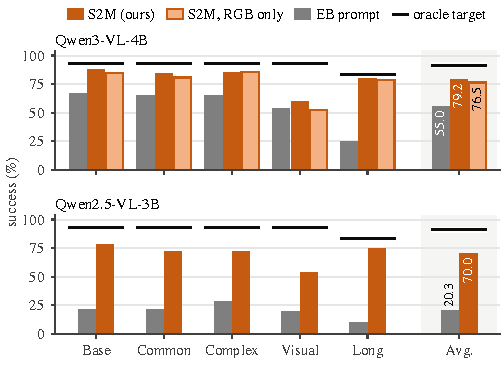
\includegraphics[width=0.7\linewidth]{figures/results.pdf}
\caption[Success with the same local model]{EB-Navigation test success with the same local model (60 episodes per
subset). Black line: geometric planner given the true target position (oracle target). The RGB-only configuration
was run with Qwen3-VL-4B.}
\label{fig:results}
\end{figure}

With Qwen3-VL-4B, \ours succeeds in \nSThree\% of the episodes against \nEBThree\% for the EB prompt, a paired gain of
\nGainThree{} percentage points (95\% CI [${+}\nGainThreeLo$, ${+}\nGainThreeHi$], $p\nGainThreeP$). Over three test
runs its average success ranges from \nSThreeMin\% to \nSThreeMax\% (standard deviation \nSThreeSD{} percentage
points), and the two RGB-only runs differ by a similar amount. Per episode, compared with the first run of \ours, the
EB prompt solves \nDiscThreeLosses{} episodes that \ours fails and fails \nDiscThreeWins{} that \ours solves; with
Qwen2.5-VL-3B the counts are \nDiscTwoLosses{} and \nDiscTwoWins. Every single run of \ours is significantly better
than the EB prompt (exact McNemar test, largest $p\nMcNThreeWorst$).
With Qwen2.5-VL-3B, \ours reaches \nSTwo\% against \nEBTwo\% (${+}\nGainTwo$\,pp, CI [${+}\nGainTwoLo$,
${+}\nGainTwoHi$]). \Cref{fig:subsets} shows the
success of every configuration on each subset, from the prompted agent to the oracle, and \cref{tab:ci} gives the
confidence interval of every configuration run on EB-Navigation and of the paired differences on which the
conclusions rest. Scaling the benchmark's agent tenfold within a model family buys \nScaleQwen{} percentage points
(Qwen2.5-VL, 7B to 72B) and \nScaleIntern{} (InternVL3, 8B to 78B); changing the role of a 4B model buys as much, and
closes \nGapClosed\% of the gap between the EB prompt and the oracle planner. The gain follows each of the four
predictions.

\begin{table}[htbp]
\centering\small
\caption[Confidence intervals of the EB-Navigation results]{EB-Navigation test success of the configurations run
in this thesis, and paired differences, with 95\% bootstrap confidence intervals and sign-flip permutation
$p$-values (\cref{sec:pre-protocol}).}
\label{tab:ci}
\begin{tabular*}{\linewidth}{@{\extracolsep{\fill}}llrcl@{}}
\toprule
Configuration & Model & Success (\%) & 95\% CI & \\
\midrule
EB prompt & Qwen3-VL-4B & \nEBThree & [\nEBThreeLo, \nEBThreeHi] & \\
Modular, single view & Qwen3-VL-4B & \nModThree & [\nModThreeLo, \nModThreeHi] & \\
\ours & Qwen3-VL-4B & \nSThree & [\nSThreeLo, \nSThreeHi] & \\
\ours, RGB only & Qwen3-VL-4B & \nRGBThree & [\nRGBThreeLo, \nRGBThreeHi] & \\
EB prompt & Qwen2.5-VL-3B & \nEBTwo & [\nEBTwoLo, \nEBTwoHi] & \\
\ours & Qwen2.5-VL-3B & \nSTwo & [\nSTwoLo, \nSTwoHi] & \\
Oracle target & true position & \nOracle & [\nOracleLo, \nOracleHi] & \\
\midrule
Paired difference & Model & $\Delta$ (pp) & 95\% CI & $p$\\
\midrule
\ours $-$ EB prompt & Qwen3-VL-4B & ${+}\nGainThree$ & [${+}\nGainThreeLo$, ${+}\nGainThreeHi$] & $\nGainThreeP$\\
\ours $-$ modular, single view & Qwen3-VL-4B & ${+}\nSOverMod$ & [${+}\nSOverModLo$, ${+}\nSOverModHi$] & $\nSOverModP$\\
Modular, single view $-$ EB prompt & Qwen3-VL-4B & ${+}\nModOverEB$ & [${+}\nModOverEBLo$, ${+}\nModOverEBHi$] & $\nModOverEBP$\\
\ours, RGB only $-$ EB prompt & Qwen3-VL-4B & ${+}\nGainRGB$ & [${+}\nGainRGBLo$, ${+}\nGainRGBHi$] & $\nGainRGBP$\\
\ours, RGB only $-$ \ours & Qwen3-VL-4B & $\nGapRGB$ & [$\nGapRGBLo$, ${+}\nGapRGBHi$] & $\nGapRGBP$\\
\ours $-$ EB prompt & Qwen2.5-VL-3B & ${+}\nGainTwo$ & [${+}\nGainTwoLo$, ${+}\nGainTwoHi$] & $\nGainTwoP$\\
Oracle $-$ \ours & Qwen3-VL-4B & ${+}\nGapOracle$ & [${+}\nGapOracleLo$, ${+}\nGapOracleHi$] & $\nGapOracleP$\\
\bottomrule
\end{tabular*}
\end{table}

\begin{figure}[htbp]
\centering
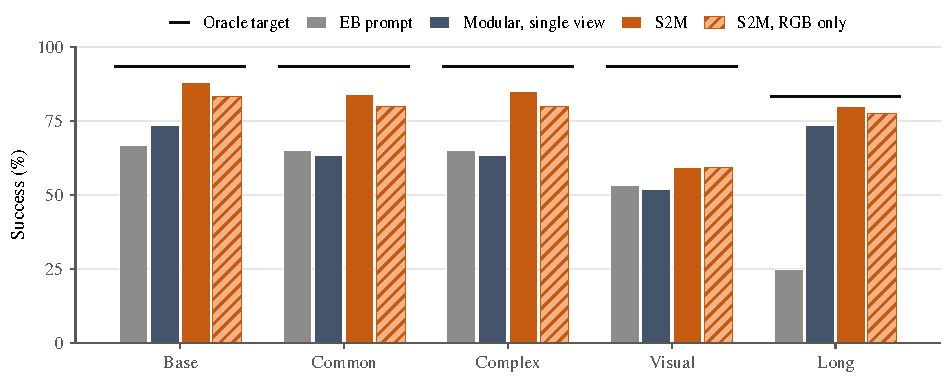
\includegraphics[width=\linewidth]{figures/th_subsets.pdf}
\caption[Success per subset]{EB-Navigation test success per subset with Qwen3-VL-4B, from the benchmark's agent to
the oracle (black line). \ours closes most of the gap to the oracle on every subset except Visual.}
\label{fig:subsets}
\end{figure}

\subsection{Prediction (i): the diagnosed failures collapse}
\Cref{fig:analysis}b breaks the failures down by outcome. Never-seen and blocked episodes fall by \nNeverRed{} and
\nBlockedRed\%, near misses by \nNearRed\%, and lost targets by \nLostRed\%. Per run, \ours never sees the target in \nNeverSThree{}
episodes (EB prompt: \nNeverEBThree), is blocked in \nBlockedSThree{} (\nBlockedEBThree), loses a seen target in
\nLostSThree{} (\nLostEBThree), and ends near it in \nNearSThree{} (\nNearEBThree). The look-around, the occupancy map,
and the memory remove the never-seen and blocked failures almost entirely and reduce the lost-after-seen ones, as
predicted. \Cref{tab:taxonomy,fig:outcomes} give the full taxonomy for both models. The change is the same
for both: the EB prompt spreads its failures over every category, while the failures of \ours collapse into
lost-after-seen and approach failures, most of which come from look-alikes (\cref{sec:exp-failures}).

\begin{figure}[htbp]
\centering
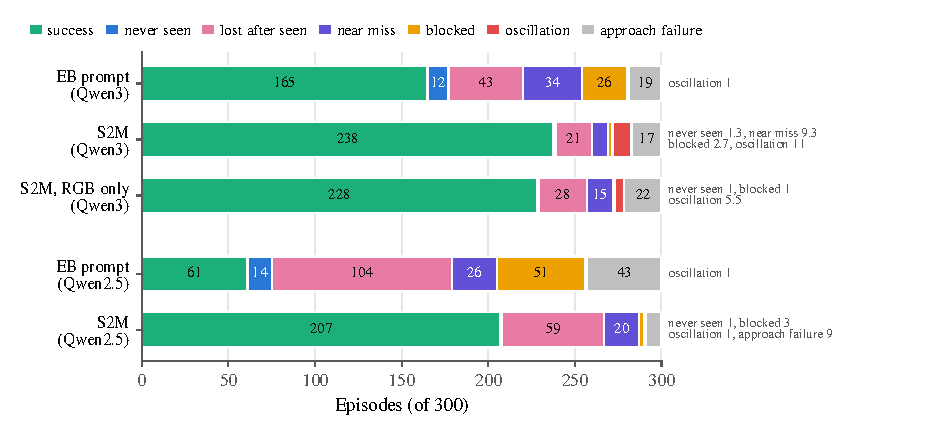
\includegraphics[width=\linewidth]{figures/th_outcomes.pdf}
\caption[Outcome of every episode]{Outcome of every EB-Navigation test episode by agent and model (first matching
rule of \cref{sec:pre-metrics}; mean over runs where a configuration was run repeatedly, so counts can be
fractional). Outcomes with fewer than 12 episodes are listed beside their bar.}
\label{fig:outcomes}
\end{figure}

\begin{figure}[htbp]
\centering
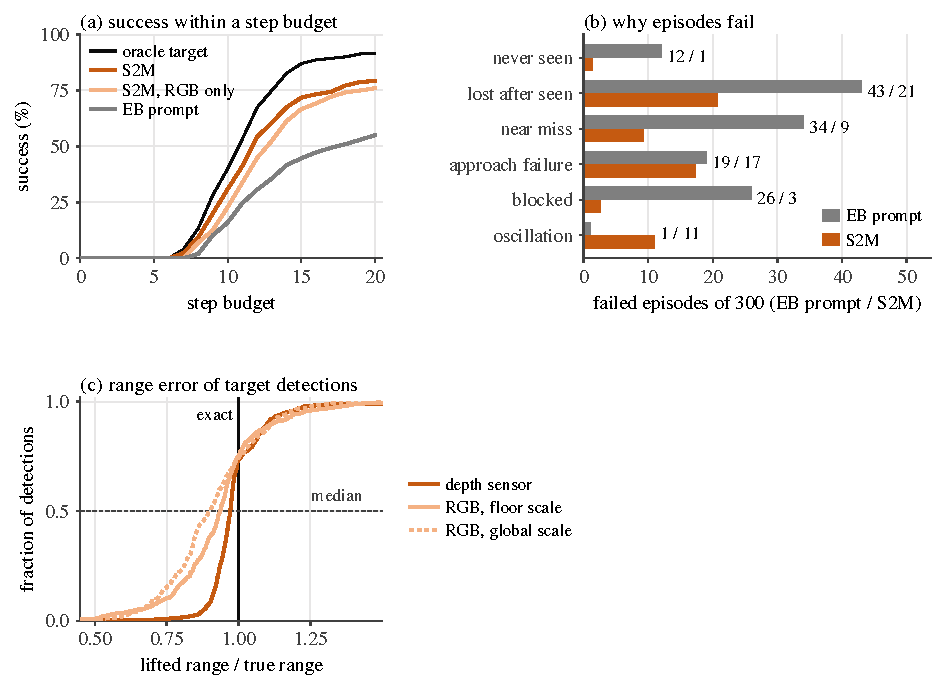
\includegraphics[width=\linewidth]{figures/analysis_thesis.pdf}
\caption[Step budget, failure outcomes, and range accuracy]{EB-Navigation test, Qwen3-VL-4B. \textbf{(a)}~Episodes
solved within a step budget, averaged over runs. \textbf{(b)}~Failed episodes by outcome (first matching rule,
\cref{sec:pre-metrics}; mean over the runs of \ours). \textbf{(c)}~Cumulative distribution of lifted over true range for
detections within 1\,m of the target (dashed: median), with the depth sensor and with monocular depth under a
per-frame floor scale (\cref{eq:floorscale}) or a global scale.}
\label{fig:analysis}
\end{figure}

\begin{table}[htbp]
\centering\small
\caption[Outcomes on EB-Navigation]{Outcomes on EB-Navigation test (episodes of 300; mean over runs where a
configuration was run repeatedly).}
\label{tab:taxonomy}
\begin{tabular*}{\linewidth}{@{\extracolsep{\fill}}lrrrrr@{}}
\toprule
& \multicolumn{3}{c}{Qwen3-VL-4B} & \multicolumn{2}{c}{Qwen2.5-VL-3B}\\
\cmidrule(lr){2-4}\cmidrule(l){5-6}
Outcome & EB prompt & \ours & \ours, RGB & EB prompt & \ours\\
\midrule
success & 165 & 237.7 & 228 & 61 & 207\\
never seen & 12 & 1.3 & 1 & 14 & 1\\
lost after seen & 43 & 20.7 & 28 & 104 & 59\\
near miss & 34 & 9.3 & 15 & 26 & 20\\
blocked & 26 & 2.7 & 1 & 51 & 3\\
oscillation & 1 & 11 & 5.5 & 1 & 1\\
approach failure & 19 & 17.3 & 21.5 & 43 & 9\\
\bottomrule
\end{tabular*}

\end{table}

\subsection{Prediction (ii): the largest gain on Long}
The gain is largest where the target starts behind the agent. On Long, \ours succeeds in \nSThreeLong\% against
\nEBThreeLong\%, only \nOracleGapLong{} percentage points below the oracle. On Base, Common, and Complex the gain is
$\nGainThreeBase$, $\nGainThreeCommon$, and $\nGainThreeComplex$ percentage points.

\subsection{Prediction (iii): the smallest gain on Visual}
On Visual the difference is not significant with Qwen3-VL-4B ($\nGainThreeVisual$\,pp, CI $[\nVisDiffLo, \nVisDiffHi]$,
$p\nVisDiffP$), and Visual is also the subset with the smallest gain with Qwen2.5-VL-3B ($\nGainTwoVisual$\,pp). This
is the subset on which single-view recognition was weakest (\cref{sec:diag-probe}); \cref{sec:exp-gap} examines it.

\subsection{Prediction (iv): far less dependence on model size}
Replacing Qwen3-VL-4B by Qwen2.5-VL-3B costs \ours \nScaleDrop{} percentage points and the EB prompt \nScaleDropEB{}
percentage points.
The smaller model loses much of its ability to plan in text, but its answers to per-image questions remain good
enough for the memory to use.
\IfFileExists{chapters/generated/qwen2b_text.tex}{The smallest model of the same family tests the prediction further. With Qwen3-VL-2B, \ours succeeds in \nSQTwo\% of the episodes and the EB prompt in \nEBQTwo\% (${+}\nGainQTwo$\,pp, CI [${+}\nGainQTwoLo$, ${+}\nGainQTwoHi$], $p\nGainQTwoP$). Halving the model from 4B to 2B costs \ours \nDropSQTwo{} percentage points and the EB prompt \nDropEBQTwo. From RGB alone, with the same monocular depth and dead reckoning as the 4B configuration, the 2B agent reaches \nRGBQTwo\%. The EB prompt with this model was run with the length-bounded output schema, which a development comparison chose over the official one, as for Qwen2.5-VL-3B (\cref{sec:pre-protocol}).
}{}

\section{Comparison with published agents}
\label{sec:exp-published}
\Cref{fig:landscape} places \ours among the agents of \cref{tab:main} by the size of their model. Even from RGB alone
(\nRGBThree\%), with a 4B model and no training, \ours exceeds every prompted MLLM up to GPT-4o,
\nNTrainFreeBelowRGB{} of the \nNTrainFree{} training-free agents, which build on GPT-4o and 8--32B
models~\cite{huang2025esca,wang2026mosaic,ju2026embodiskill,ma2026brainmem,lee2026emho,liang2026robofoundry}, and MuSix
and SVA, which train extra models around a 4B policy~\cite{jang2026musix,xie2026sva}. MuSix and SVA report episodes
36--60 and 37--60 of each subset, on which \ours (RGB only) reaches \nRGBMuSix{} and \nRGBSVA\%; EMHO reports its
best held-out score over search iterations on half of each subset. Only the tool-library
agents~\cite{zhou2026enabling} and RoboFoundry on GPT-6 Astra, which rewrites its prompts and code on the test
episodes, score higher. These comparisons use the results reported by the respective authors.

\begin{figure}[htbp]
\centering
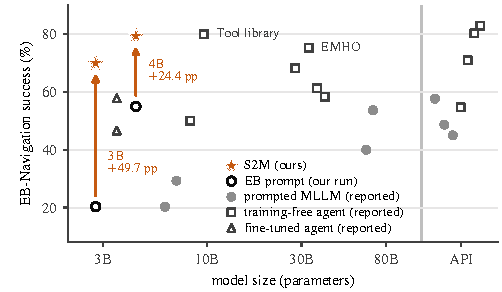
\includegraphics[width=0.7\linewidth]{figures/landscape.pdf}
\caption[Success against model size]{EB-Navigation success against model size (\cref{tab:main}). Arrows: gain of
\ours over the EB prompt with the same model; closed models share the API column.}
\label{fig:landscape}
\end{figure}

\section{Modularity alone is not enough}
\label{sec:exp-modular}
A modular structure removes the model from planning, but it does not by itself make the model's answers reliable.
The modular agent of \cref{sec:exp-setup} is \ours without multi-view fusion and the crop check: the same model,
map, planner, look-around, exploration, and exhaustion, acting on single-view detections. It reaches \nModThree\%, \nModOverEB{} percentage points above the EB prompt
($p\nModOverEBP$) but \nSOverMod{} below \ours (CI [${+}\nSOverModLo$, ${+}\nSOverModHi$], $p\nSOverModP$). Its gain
over the EB prompt falls almost entirely on Long ($\nModOverEBLong$\,pp), where the look-around alone finds the target;
on the other subsets it is level with the EB prompt. On Base, Common, and Complex, \ours exceeds the modular agent by $\nSOverModBase$,
$\nSOverModCommon$, and $\nSOverModComplex$ percentage points: these are the subsets in which the agent starts facing
the target and must hold on to it while approaching, which a single-view agent cannot do when the model places a
false box. Moving the state out of the model therefore gives part of the gain, and the evidence design for a
generative sensor gives the rest.

\section{Ablation of components}
\label{sec:exp-ablation}
\Cref{tab:abl} changes one element of \ours at a time and compares each variant with the full model over the same
episodes.

\begin{table}[t]
\centering\small
\setlength{\tabcolsep}{6pt}
\caption{Components and sensing on EB-Navigation test (Qwen3-VL-4B). $\Delta$: paired difference from the full model; $p$: sign-flip permutation test, Holm-corrected. Bold: significant.}
\label{tab:abl}
\resizebox{\linewidth}{!}{\begin{tabular}{@{}lrrrrrrrlr@{}}
\toprule
Variant & Base & Common & Complex & Visual & Long & Avg. & \multicolumn{2}{c}{$\Delta$ (95\% CI)} & $p$\\
\midrule
\ours (full) & 87.8 & 83.9 & 85.0 & 59.4 & 80.0 & 79.2 & \multicolumn{3}{c}{reference}\\
\midrule
\multicolumn{10}{@{}l}{\textit{Components}}\\
w/o fusion & 78.3 & 75.0 & 78.3 & 43.3 & 78.3 & 70.7 & $\mathbf{-8.6}$ & {\footnotesize[$-12.7$, $-4.6$]} & $3.4{\times}10^{-4}$\\
w/o look-around & 95.0 & 90.0 & 91.7 & 73.3 & 46.7 & 79.3 & $+0.1$ & {\footnotesize[$-4.2$, $+4.6$]} & $1.00$\\
w/o exhaustion & 86.7 & 81.7 & 85.0 & 58.3 & 76.7 & 77.7 & $-1.6$ & {\footnotesize[$-3.6$, $+0.3$]} & $0.38$\\
w/o crop check & 81.7 & 78.3 & 80.0 & 58.3 & 75.0 & 74.7 & $\mathbf{-4.6}$ & {\footnotesize[$-7.9$, $-1.3$]} & $0.04$\\
\midrule
\multicolumn{10}{@{}l}{\textit{Sensing}}\\
odometry noise (5\%, 2$^\circ$) & 90.0 & 88.3 & 88.3 & 60.0 & 81.7 & 81.7 & $+2.4$ & {\footnotesize[$-0.4$, $+5.4$]} & $0.38$\\
RGB only, global scale & 65.0 & 65.0 & 60.0 & 38.3 & 55.0 & 56.7 & $\mathbf{-22.6}$ & {\footnotesize[$-28.4$, $-16.8$]} & ${<}10^{-5}$\\
RGB only, floor scale & 83.3 & 80.0 & 80.0 & 59.2 & 77.5 & 76.0 & $-3.2$ & {\footnotesize[$-6.7$, $+0.2$]} & $0.31$\\
\bottomrule
\end{tabular}}
\end{table}


\Cref{fig:forest} shows the same differences with their confidence intervals. Two variants stand apart from the
rest: removing fusion and replacing the per-frame floor scale by a global one. The intervals of all other variants
include zero.

\begin{figure}[htbp]
\centering
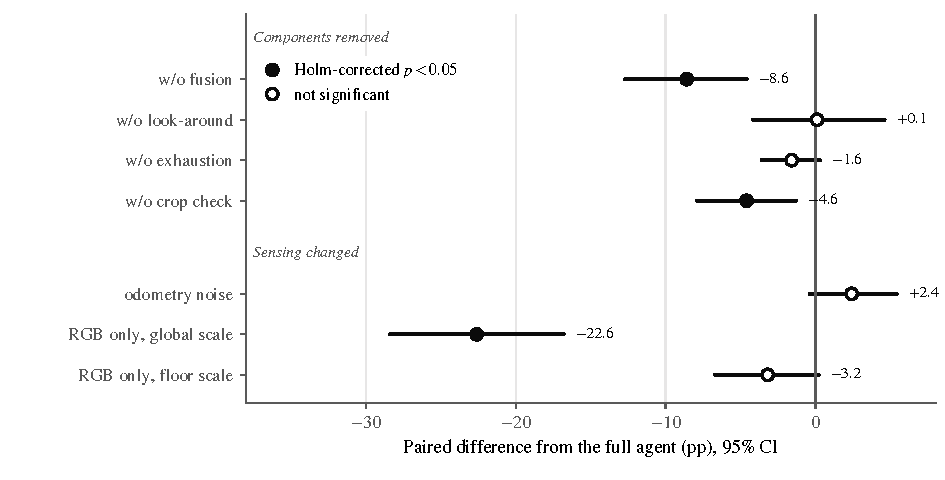
\includegraphics[width=\linewidth]{figures/th_forest.pdf}
\caption[Ablations with confidence intervals]{Paired difference in EB-Navigation success between each variant and
the full agent (Qwen3-VL-4B), with 95\% bootstrap intervals. Filled marker: significant after Holm correction ($p<0.05$); open marker: not
significant.}
\label{fig:forest}
\end{figure}

\subsection{Fusion keeps a found target}
Disabling multi-view fusion, so that each detection replaces the earlier hypotheses, lowers success by
\nAblFusionAbs{} percentage points (Holm $p\nAblFusionP$), the largest effect of any component. Fusion does not help the agent find the target: \nDetPrec\% of single lifted detections lie within
0.5\,m of it, and a hypothesis there reaches commitment in \nHoldNF{} episodes without fusion and \nHoldS{} with it.
Fusion keeps the target once found. Without it, each detection, including the false boxes of \cref{sec:diag-probe},
replaces the committed hypothesis, and lost targets rise from \nLostSThree{} to \nLostNF{} episodes and near misses
from \nNearSThree{} to \nNearNF.

\subsection{The look-around trades Long against the other subsets}
Removing the look-around leaves the average unchanged ($\nAblScan$\,pp) but changes Long by $\nAblScanLong$\,pp,
because the agent no longer turns to find a target behind it. The other subsets gain $\nAblScanOtherMin$ to
$\nAblScanOtherMax$\,pp, the steps that the turn no longer costs. On Long, \nScanLongFull{} episodes succeed only with
the look-around and \nScanLongAbl{} only without it (McNemar $p\nScanLongP$). The look-around is therefore what makes
the agent robust to where it starts. The inspection rule of \cref{sec:method-search} lowered this cost on the
development split, but on the test set the two sides still balance.

\subsection{The crop check and exhaustion}
Removing the crop check lowers success by \nAblZoomAbs{} percentage points (Holm $p\nAblZoomP$); it costs VLM calls,
not environment steps. Removing exhaustion changes success by $\nAblExhaust$\,pp (Holm $p\nAblExhaustP$). It acts only after the agent has
reached a look-alike: in \nExhVisLo--\nExhVisHi{} Visual episodes per run, where appearance-only goals produce
look-alikes that must be ruled out once visited, and in \nExhOtherLo--\nExhOtherHi{} on each other subset.

\section{One RGB camera is enough}
\label{sec:exp-sensing}
\label{sec:sensing}
\subsection{Pose}
Dead reckoning (\cref{eq:deadreckon}) is exact in heading and tilt. Its position error along the test trajectories,
caused by the simulator's grid snapping, averages \nDRmean\,m. Accumulated odometry noise of 5\% per translation and
2$^\circ$ per turn changes success by $\nAblOdom$ percentage points (\cref{tab:abl}).

\subsection{Depth}
Monocular depth with one global scale $\bar\sigma$ is not enough. With pose from the executed actions, \ours then
reaches \nRGBGlobal\%, level with the EB prompt ($\nGainGlobal$\,pp, $p\nDiscGlobalP$). The global scale places target
detections at a median \nRangeGlobal{} of their true range (\cref{fig:analysis}c) and lifts \nBlockGlobal\% of the
nearby floor above the obstacle threshold, so the agent walks to a point short of the target: \nShortGlobal{} failures
exhaust a hypothesis within 1\,m of it, none with the sensor. The per-frame floor scale (\cref{eq:floorscale}) lowers
the falsely blocked floor to \nBlockFloor\% and moves the range ratio to \nRangeFloor{} (sensor: \nRangeSensor).
Success rises to \nRGBThree\%, \nGainRGB{} percentage points above the EB prompt ($p\nGainRGBP$) and \nGapRGBAbs{}
below the depth sensor (Holm $p\nAblRgbfloorP$).

\section{Efficiency and cost}
\label{sec:exp-efficiency}
\ours also reaches the target in fewer steps. On the \nStepN{} episodes that both agents solve in every run, it needs
\nStepS{} steps against \nStepEB{} ($p\nStepP$). Within ten and fifteen steps it solves \nBudSTen{} and \nBudSFifteen\%
of the episodes against \nBudEBTen{} and \nBudEBFifteen\% for the EB prompt (\cref{fig:analysis}a).

The cost of an episode is spent differently. \ours makes \nCallsS{} VLM calls per episode against \nCallsEB{} for the
EB prompt, but each call asks one short question: it reads \nTokS{}k prompt tokens and generates \nTokSc{} tokens per
episode, against \nTokEB{}k and \nTokEBc{}k for the EB prompt, whose plans and reasoning dominate its generation.
Because generation is the slow part of decoding, many short questions are cheaper than a few long plans on a small
GPU. On the RTX 5060, which also renders the simulator, \ours takes \nSecS\,s per step and \tTimeEpS\,s per
episode on average, including rendering, all VLM calls, mapping, and planning, against \nSecEB\,s per step for the EB
prompt, \nSpeedUp{} times longer. The RGB-only configuration, which runs the depth network on the CPU, takes
\nSecRGB\,s per step. This is fast enough for a robot that moves 0.25\,m per step.

\section{Qualitative analysis}
\label{sec:exp-qualitative}
\Cref{fig:traj} shows three test episodes chosen by fixed rules, the first matching episode in index order of each
subset. In the Long episode (a), the EB prompt never turns toward the target, while \ours completes its look-around,
finds the target, and reaches it. In the Base episode (b), furniture blocks the EB prompt, which repeats rejected
moves; \ours plans around the obstacle on its map. In the Visual episode (c), \ours proposes only look-alikes and
fails while the EB prompt succeeds, an example of the recognition limit discussed next.

\begin{figure}[t]
\centering
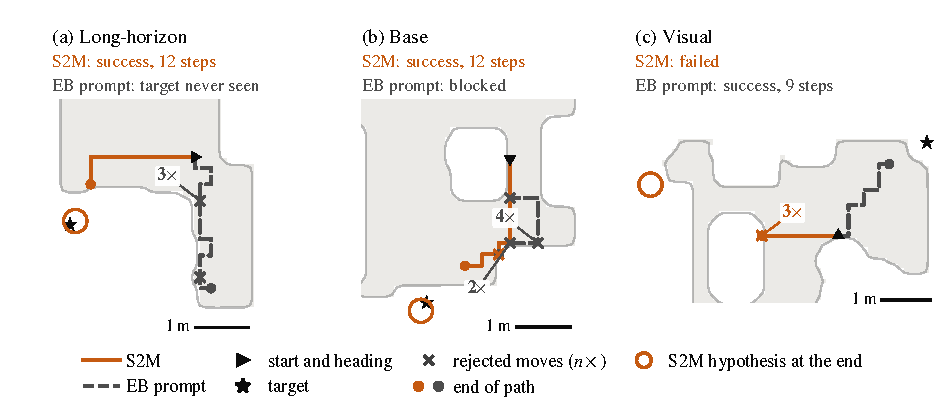
\includegraphics[width=\textwidth]{figures/trajectories_thesis.pdf}
\caption{Trajectories on three EB-Navigation test episodes (Qwen3-VL-4B) and the hypotheses of \ours at the end of each. Grey: reachable floor; targets on furniture lie outside it. $n\times$: rejected moves at one spot. (a)~the target starts behind the agent; (b)~furniture blocks the EB prompt; (c)~\ours proposes only look-alikes.}
\label{fig:traj}
\end{figure}


\Cref{fig:episode} looks inside one successful episode, the Long-horizon episode of \cref{fig:arch,tab:trace}. The
camera frames show what the VLM sees and where it places its box, and the plot below shows how the evidence of each
hypothesis develops. The agent turns away from an empty wall (step 0), sees the alarm clock and commits to it as
soon as it appears (step 2), keeps it while the model briefly boxes a look-alike (step 7), and reaches it with high
evidence (step 13). The look-alikes never approach the commit threshold.

\begin{figure}[htbp]
\centering
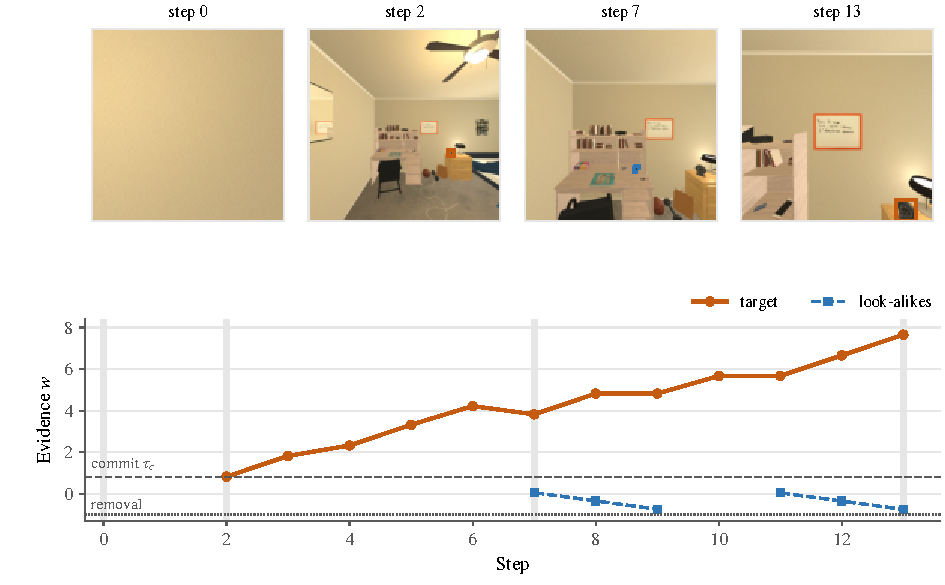
\includegraphics[width=\linewidth]{figures/th_episode.pdf}
\caption[Inside one episode]{Inside one Long-horizon test episode of \ours (Qwen3-VL-4B, target: alarm clock).
Top: camera frames at four steps, re-rendered from the saved trajectory, with the VLM's box (orange solid: on the
target; white: on a look-alike). Bottom: evidence of every hypothesis over the episode; grey bands and bold
step numbers mark the frames shown above. The episode ends in success after step 13, before either look-alike reaches
the removal line.}
\label{fig:episode}
\end{figure}

\section{The remaining failures of \ours}
\label{sec:exp-failures}
The failures that remain are of a different kind from those of the EB prompt. \Cref{tab:taxonomy} shows that \ours
almost never fails to see the target or gets blocked; its largest remaining category is \emph{lost after seen}, with
\tLostSAll{} episodes per run. Of these, \tLostSVisual{} fall on Visual, where the agent ``sees'' a look-alike that it
has proposed in place of the target and the true target is visible only in passing. Outside Visual, \ours loses a seen
target in a few episodes per subset. Near misses (\nNearSThree{} per run) and approach failures are also concentrated on Visual,
where the agent approaches a candidate that is not the target. With Qwen2.5-VL-3B, lost-after-seen is the largest failure mode for both agents, but \ours reduces it
from \nLostEBTwo{} to \nLostSTwo{} episodes.

\section{The remaining gap: appearance-only goals}
\label{sec:exp-gap}
Visual is the weakest subset in every run of \ours (\nVisSRLo--\nVisSRHi\%), accounts for \nVisGapShare\% of the gap to
the oracle, and is the only subset on which the gain over the EB prompt is not significant. The failure is recognition. A
candidate comes within 0.5\,m of the target in \nRecallOtherLo--\nRecallOtherHi\% of the episodes of every other subset
but in only \nRecallVisLo--\nRecallVisHi\% of the Visual ones, and \nVisFailNoCand{} of the \nVisFail{} Visual failures
never produce one. No memory can recover a target that the sensor never proposes; this limit lies in the model.

\section{RoboTHOR ObjectNav}
\label{sec:exp-robothor}
On the full RoboTHOR validation split, \ours reaches \nRoboSR\% success (CI [\nRoboSRLo, \nRoboSRHi]) and \nRoboSPL\%
SPL. \Cref{tab:robothor} compares it with published methods. Among zero-shot methods its success rate is below only
ForesightNav, which uses a 12B model~\cite{liu2026foresightnav}, and STRIVE, which uses Gemini-2.0-flash with a
detector~\cite{zhu2025strive}; its SPL is second only to STRIVE and above that of the ProcTHOR policy trained for the
task~\cite{deitke2022procthor}. Success ranges from \nRoboWorst\% (vases) to \nRoboBest\% (basketballs) by category
(\cref{fig:robothor}). \nRoboErr{} of the episodes end because the simulator rejects the start pose and are counted as
failures.

\subsection{How RoboTHOR episodes end}
RoboTHOR adds the decision to stop, so failures can come from stopping at the wrong place or from never stopping.
\Cref{fig:robothor-outcomes} separates the two. The agent issues Stop in \tRStop{} episodes, and \tRStopOk{} of these
succeed, a stop precision of \tRStopPrec\%. Of the \tRWrong{} wrong stops, \tRWrongNear{} end within 1.5\,m of the
target and the median one ends \tRWrongDist\,m away, so most wrong stops are at a look-alike rather than just short of
the target. In \tRLimit{} episodes the agent uses all 500 steps without stopping. In \tRLimitAppr{} of them it does
commit to and approach a candidate, but the stop check of \cref{sec:method-stop} rejects it (\tRLimitRej{} rejections
in total), so the agent exhausts the candidate and keeps searching; on average it spends \tRLimitExpl\% of these
episodes exploring. The stop check therefore trades wrong stops for unfinished episodes. Both failure types trace back to recognition: a look-alike that passes the stop check produces a wrong stop,
and a target that fails it produces an unfinished episode. With a model that tells targets from look-alikes more
reliably, the same agent would convert both into successes. Successful episodes take \tRStepsSucc{} steps at the median, and the agent runs at
\tRTimeStep\,s per step with \tRCallsEp{} VLM calls per episode.

\Cref{fig:robothor-budget} shows when the successes come and how the stop check decides. Success reaches
\tRBudHundred\% within 100 steps and \tRBudTwoHundred\% within 200, against \nRoboSR\% at the 500-step limit; nine in
ten successful episodes end within \tRStepsPninety{} steps. The last 300 steps therefore add only a few points: an
episode that has not found its target by then has usually committed to the wrong object or explored the wrong part of
the apartment. The stop check separates its two outcomes sharply: \tRCheckSure\% of its \tRCheckN{} presence answers lie below 0.1
or above 0.9, so the threshold of 0.5 is not a fine-tuned boundary.
The check rejects \tRRejN{} candidates in \tRRejEp{} episodes, and \tRRejEpOk{} of these episodes still succeed
after the agent moves on, which is the purpose of exhaustion on a benchmark that ends an episode only on Stop.

\begin{figure}[htbp]
\centering
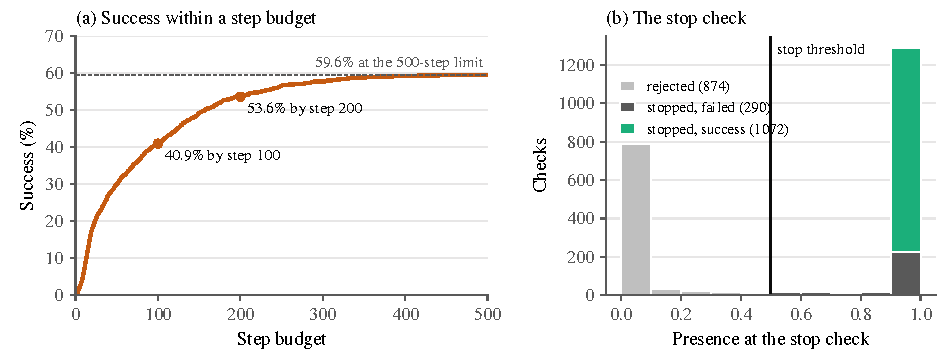
\includegraphics[width=\linewidth]{figures/th_robothor_budget.pdf}
\caption[RoboTHOR step budget and stop check]{RoboTHOR validation, \ours with Qwen3-VL-4B. \textbf{(a)}~Episodes
solved within a step budget, of all \nRoboN. \textbf{(b)}~Presence probability of the fresh query at every stop check,
by its outcome.}
\label{fig:robothor-budget}
\end{figure}

\begin{figure}[htbp]
\centering
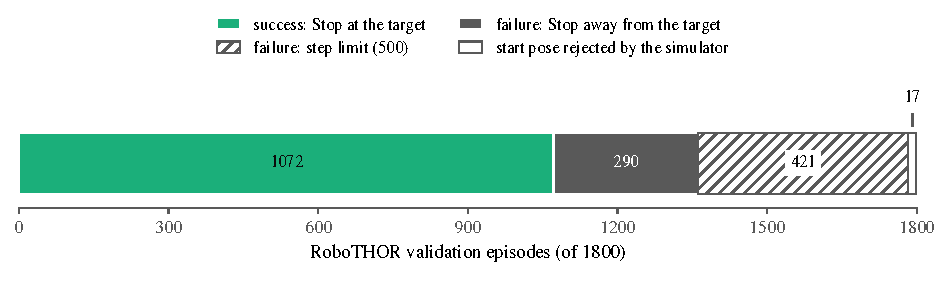
\includegraphics[width=\linewidth]{figures/th_robothor_outcomes.pdf}
\caption[How RoboTHOR episodes end]{How the \nRoboN{} RoboTHOR validation episodes of \ours end.}
\label{fig:robothor-outcomes}
\end{figure}

\begin{table}[!tb]
\centering\small
\caption{RoboTHOR ObjectNav validation (\nRoboN{} episodes), SR and SPL in \%. Bold: best; underlined: second.
$^\flat$As reported by SG-Nav~\cite{yin2024online}.}
\label{tab:robothor}
\begin{tabular*}{\linewidth}{@{\extracolsep{\fill}}llcrr@{}}
\toprule
Method & Input & Year & SR & SPL \\
\midrule
\multicolumn{5}{@{}l}{\textit{Zero-shot}}\\
CoW~\cite{gadre2022cows} & RGB-D & 2022 & 26.7 & 16.9 \\
LGX~\cite{dorbala2024lgx} & RGB-D & 2024 & 35.0 & 21.9 \\
ESC~\cite{zhou2023esc} & RGB-D & 2023 & 38.1 & 22.2 \\
L3MVN$^\flat$~\cite{yu2023l3mvn} & RGB-D & 2023 & 41.2 & 22.5 \\
VLFM$^\flat$~\cite{yokoyama2023vlfm} & RGB-D & 2023 & 42.3 & 23.0 \\
OpenFMNav$^\flat$~\cite{kuang2024openfmnav} & RGB-D & 2024 & 44.1 & 23.3 \\
SG-Nav~\cite{yin2024online} & RGB-D & 2024 & 47.5 & 24.0 \\
UniGoal~\cite{yin2025unigoal} & RGB-D & 2025 & 48.0 & 24.2 \\
CogNav~\cite{cao2024cognav} & RGB-D & 2024 & 54.6 & 24.3 \\
MVP-Nav~\cite{xie2026mvpnav} & RGB & 2026 & 57.5 & 26.8 \\
ForesightNav~\cite{liu2026foresightnav} & RGB-D & 2026 & 62.5 & 32.9 \\
STRIVE~\cite{zhu2025strive} & RGB-D & 2025 & \textbf{68.1} & \textbf{36.3} \\
\multicolumn{5}{@{}l}{\textit{Trained for the task}}\\
ProcTHOR~\cite{deitke2022procthor,gadre2022cows} & RGB & 2022 & \underline{66.4} & 27.4 \\
\midrule
\ours (Qwen3-VL-4B) & RGB-D & this work & \nRoboSR & \underline{\nRoboSPL} \\
\bottomrule
\end{tabular*}
\end{table}


\begin{figure}[htbp]
\centering
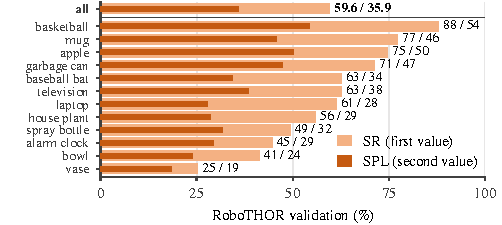
\includegraphics[width=0.7\linewidth]{figures/robothor_cats.pdf}
\caption{\ours on RoboTHOR validation by target category.}
\label{fig:robothor}
\end{figure}

\section{Summary}
The experiments confirm all four predictions of the diagnosis. With the same model, \ours gains as much as a tenfold
larger model gives the benchmark's agent, removes the never-seen and blocked failures and halves lost targets, gains
most on Long and least on Visual, and loses far less when the model shrinks. A modular agent with the same model recovers only part of the gain; multi-view fusion supplies most of the rest. The
agent works from RGB alone, uses fewer steps and \nSpeedUp{} times less time per step, and transfers to RoboTHOR. Its main remaining limit is the recognition
of objects described only by appearance.


\chapter{Conclusions}
\label{chap:conclusions}

\section{Answers to the research questions}
\noindent\textbf{RQ1: Why do small VLMs fail as navigation agents?} Because the agents they are placed in make them
keep spatial state in generated text. Controlled experiments on the same episodes ruled out the two other causes: a
geometric planner given the target position solves \nOracle\% of the EB-Navigation test episodes, and Qwen3-VL-4B
places a correct box on a visible named target in \nProbeThreeCommon--\nProbeThreeBase\% of single views. The
failures of the prompted agent are failures of state: it loses seen targets, collides with furniture, and does not
turn toward a target behind it (\cref{chap:diagnosis}).

\noindent\textbf{RQ2: What should an agent built around a small VLM look like?} It should ask the model only what
the current image can settle and keep everything else in metric form. \ours does so with two per-image questions, a
hypothesis memory, a search rule, and an occupancy-map planner (\cref{chap:method}). Of its components, multi-view
evidence fusion carries the gain: a generic modular agent that acts on single-view answers trails \ours by
\nSOverMod{} percentage points, and removing fusion alone costs \nAblFusionAbs{} (\cref{sec:exp-modular,sec:exp-ablation}).

\noindent\textbf{RQ3: How far does this agent close the gap to larger models?} With a 4-bit 4B model on one 8\,GB GPU
and without training, \ours succeeds in \nSThree\% of the EB-Navigation test episodes, \nGainThree{} percentage
points more than the benchmark's agent with the same model. From RGB alone it reaches \nRGBThree\%, which is above
both fine-tuned 4B agents and seven of ten training-free agents built on 8B to frontier-scale models. With a smaller
3B model the gain grows to \nGainTwo{} percentage points, and on RoboTHOR \ours reaches \nRoboSR\% success, above ten
published zero-shot methods (\cref{chap:experiments}).

\section{Discussion}
The central finding of the thesis is that, for small models, the role matters more than the model. Agents designed
around frontier models ask the model to perceive, remember, and plan, and they degrade quickly as the model shrinks.
An agent that asks the same model only what it can see loses far less: replacing the 4B model by a 3B model costs
\ours \nScaleDrop{} percentage points and the benchmark's agent \nScaleDropEB. The division of labor between a
semantic sensor and a metric controller is old in robotics, but the thesis shows that a generative VLM needs more
than this division: because its single answers are unreliable, the controller must treat them as evidence and
accumulate them over distinct viewpoints.

\subsection{Implications for the design of robot agents}
Three lessons from this thesis apply beyond EB-Navigation.

\noindent\textbf{Match the question to the model.} A question about the current image is one a small model can
answer and an agent can check. A question about the room, the history, or the plan is one it cannot. Agent designs
that pass the whole problem to the model test the model's ability to plan, not its ability to see. For small models
the second is far stronger than the first.

\noindent\textbf{Treat a generative model as a noisy sensor.} A generative VLM places boxes in views that do not
show the target and repeats its answers from the same viewpoint. An agent should therefore weigh its answers, combine
them across viewpoints, and lower them when the expected detection does not appear, as one would with any other
noisy sensor. Of all components of \ours, this evidence fusion is the one whose removal costs most.

\noindent\textbf{Keep geometry in geometry.} Distances, free space, and directions already looked at are exact
quantities that classical methods compute reliably from depth and pose, or from RGB alone with a ground-plane scale.
There is no reason to ask a language model to estimate them in words.

\section{Limitations}
\noindent\textbf{Task scope.} The controller of \ours is written for one task, reaching one object. A prompted agent
can be redirected to a new task by changing its prompt; \ours needs a new controller.

\noindent\textbf{Scene scale.} EB-Navigation episodes take place in single rooms with at most 20 steps. On the
multi-room RoboTHOR apartments \ours remains below two zero-shot methods (\cref{tab:robothor}). Its exploration
follows geometric rules and does not use semantic priors about where objects tend to be, which matter more in larger
scenes. The components designed for competing candidates showed no significant effect in single rooms and remain
untested at a larger scale.

\noindent\textbf{Recognition.} Visual is the only subset on which \ours does not exceed the benchmark's agent. When the
instruction describes only appearance, the small model rarely proposes the target, and no memory can recover a target
that is never detected (\cref{sec:exp-gap}).

\noindent\textbf{Simulation only.} All results come from AI2-THOR. The RGB-only configuration removes the depth sensor
and the simulator pose, but its dead reckoning benefits from the simulator's discrete actions; real actuation noise,
motion blur, and lighting have not been tested.

\section{Future work}
\noindent\textbf{Deployment on a robot.} The agent needs only an RGB camera, odometry, and a 4B model on a consumer
GPU, which makes on-board deployment on a mobile or legged robot the most direct next step.

\noindent\textbf{Semantic exploration.} The VLM could also answer questions that the current image can settle about
where to search, for example which visible doorway leads toward a kitchen, without being asked to plan.

\noindent\textbf{Larger scenes and other tasks.} Multi-room benchmarks would test the memory and the search index at
a larger scale, and controllers for multi-step tasks, such as finding an object and then a receptacle, would test how
far the division of labor between a semantic sensor and a metric controller extends.

\noindent\textbf{Appearance-only goals.} Comparing several candidates within one image, rather than judging each
alone, may help a small model recognize objects described only by how they look.


\printthebibliography

\appendix
\chapter{Prompts, Parameters, and Serving}
\label{app:impl}
This appendix lists every parameter of \ours, the exact prompts, and the serving settings.

\section{Parameters}
\label{sec:appA-params}
\Cref{tab:s-params} lists every parameter of \ours. All were fixed on the development split (\cref{sec:appB-dev})
and are the same for both models and for the RGB-only configuration; RoboTHOR changes only the items of the
explicit-stopping rule of \cref{sec:method-stop}.

\begin{table}[htbp]
\centering\small
\caption{Parameters of \ours on EB-Navigation.}
\label{tab:s-params}
\footnotesize\setlength{\tabcolsep}{3pt}
\begin{tabular*}{\linewidth}{@{\extracolsep{\fill}}llr@{}}
\toprule
Group & Parameter & Value\\
\midrule
Questions & presence threshold for named targets & 0.5\\
 & crop side (times the box's longer side) & 2.5\\
 & crop and tile resolution & 448\,px\\
 & crop acceptance & 0.5\\
 & weight of a rejected crop & $0.2\,\pi^z_t$\\
Lifting & depth window (fraction of the box) & 0.5\\
 & maximum range & 6\,m\\
 & floor / obstacle height & 0.10 / 0.1--1.9\,m\\
 & occupancy grid & 5\,cm\\
Memory & association radius $r$ & 0.5\,m\\
 & repeated-view discount $\gamma$ & 0.25\\
 & same view: position, heading & 0.2\,m, equal\\
 & negative evidence $\lambda$ & 0.4\\
 & image margin, occlusion tolerance & 20\,px, 0.3\,m\\
 & removal threshold & $w_k\le-1$\\
Search & commit $\tau_c$ / keep $\tau_k$ & 0.8 / 0.4\\
 & approach a weak hypothesis & $w_k\ge0.35$\\
 & exhaustion radius & 0.9\,m\\
 & exploration goal distance & 0.75--3\,m\\
 & tiles, overlap, boxes checked & $3{\times}3$, 20\%, 4\\
Planning & cost of an unobserved edge point & 0.15\\
 & obstacle inflation (fallback) & 0.20 (0.10)\,m\\
 & goal tolerance & 0.55\,m\\
\bottomrule
\end{tabular*}
\end{table}

\section{Prompts}
\label{sec:appA-prompts}
The target phrase $s$ comes from one text-only query per episode:
\begin{quote}\small\ttfamily
A robot must navigate to one object in a house. Instruction: "$\langle\ell\rangle$"
Reply with JSON \{"name": "...", "appearance\_only": true or false, "looks": "..."\} where
- name: the most likely specific household object, as its common name in 1-2 words (e.g. "toaster", "trash can",
"laptop"; never a vague word like "device" or "object").
- appearance\_only: true if the instruction describes the object only by colour, shape, material or texture,
without saying what it is or what it is used for.
- looks: the appearance words from the instruction (colour, shape, material), empty if none.
\end{quote}
$s$ is the name, or the appearance words when \texttt{appearance\_only} is true. The two per-frame queries are
\begin{quote}\small\ttfamily
Does this image show $\langle s\rangle$? Answer yes or no.\\[0.3em]
Locate the $\langle s\rangle$ in the image and output its bounding box as JSON: [\{"bbox\_2d": [x1, y1, x2, y2],
"label": "$\langle s\rangle$"\}]. If it is not in the image, output [].
\end{quote}
The presence query generates one token and reads $P(\textit{yes})$ and $P(\textit{no})$ from the ten most likely
first tokens (\cref{eq:s-presence}). The crop check asks the presence query and each tile the box query, both on
the magnified image. Box replies are parsed with one regular expression; a box narrower than 2\,px counts as no box.
\begin{equation}
\pi_t=\frac{\sum_{y\in\textit{yes}}P(y)}{\sum_{y\in\textit{yes}}P(y)+\sum_{n\in\textit{no}}P(n)} ,
\label{eq:s-presence}
\end{equation}
where the sums run over the case variants of each answer among the ten tokens; $\pi_t=0.5$ if neither appears.

\section{Serving}
\label{sec:appA-serving}
Both models run in vLLM with their 4-bit AWQ checkpoints, temperature 0, and at most 96 generated tokens for a box
and one for a presence answer. Qwen2.5-VL receives frames resized to at most 409{,}600 pixels; Qwen3-VL uses its
default processor. The two per-frame queries are sent in parallel.


\chapter{Evaluation Protocol and Additional Results}
\label{app:results}
This appendix details the evaluation protocol and the RoboTHOR results by category.

\section{Development split}
\label{sec:appB-dev}
EmbodiedBench provides target objects and the three instruction variants for 90 iTHOR rooms, and its test set uses
60 of them (FloorPlan11--30, 211--230, 311--330). We rerun the benchmark's own generator on the other 30
(FloorPlan1--10, 201--210, 301--310): a start pose 2.5--3.0\,m from the first instance of the target with the camera
level, Common, Complex, and Visual from the same targets with the benchmark's instruction variants, and Long as Base
with the start heading rotated by 180$^\circ$. This yields five subsets of 30 targets; three generator seeds give
each target three start poses, 450 episodes in all. Every parameter of \cref{tab:s-params} and every design choice of
\cref{chap:method} was selected on this split. Each of the four components was kept only if removing it lowered
development success (paired McNemar over the 450 episodes, Holm over the four, $p<0.05$; all four had $p\le0.003$),
and the configuration was then frozen before its test runs.

\section{Statistics}
All agents run on the same 300 test episodes, so each comparison uses per-episode differences. A configuration run
several times enters with its per-episode mean success. Confidence intervals are percentile intervals of $10^4$
episode-level bootstrap resamples. $p$-values are two-sided sign-flip permutation tests with $10^6$ random sign
assignments; the seven variants of \cref{tab:abl} are Holm-corrected together. Comparisons of two single
binary runs use the exact McNemar test.

\section{Outcome categories}
A failed episode takes the first matching category: the target never enters the view; the final distance is at most
1.5\,m (near miss); the target is out of view in the last five steps (lost after seen); at least 30\% of the actions
are rejected (blocked); at least three immediate reversals (oscillation); otherwise approach failure. Visibility
comes from the simulator's object metadata.

\section{RoboTHOR episodes}
\nRoboErr{} of the \nRoboN{} validation episodes end because the simulator rejects the start pose
(\texttt{teleport failed}); they are counted as failures.

\section{RoboTHOR by category}
\Cref{tab:s-robothor} lists success and SPL for each of the twelve categories.

\begin{table}[htbp]
\centering\small
\caption{\ours on RoboTHOR validation by target category (150 episodes each).}
\label{tab:s-robothor}
\begin{tabular*}{\linewidth}{@{\extracolsep{\fill}}lrrr@{}}
\toprule
Category & Episodes & SR & SPL\\
\midrule
basketball & 150 & 88.0 & 54.3\\
mug & 150 & 77.3 & 45.7\\
apple & 150 & 74.7 & 50.1\\
garbage can & 150 & 71.3 & 47.2\\
television & 150 & 62.7 & 38.5\\
baseball bat & 150 & 62.7 & 34.4\\
laptop & 150 & 61.3 & 27.8\\
house plant & 150 & 56.0 & 28.7\\
spray bottle & 150 & 49.3 & 31.8\\
alarm clock & 150 & 44.7 & 29.5\\
bowl & 150 & 41.3 & 23.8\\
vase & 150 & 25.3 & 18.5\\
\midrule
all & 1800 & 59.6 & 35.9\\
\bottomrule
\end{tabular*}

\end{table}


\end{document}
